\chapter{Turning Climate Data into Information: Learning Meteorological Seasons}
\label{chap:climate-information}

\ifpdf
  \graphicspath{{Chapter3/Figs/}{Chapter3/Figs/PDF/}}
\else
  \graphicspath{{Chapter3/Figs/Vector/}{Chapter3/Figs/}}
\fi

\noindent\textit{Parts of this chapter are based on the work entitled \emph{A Machine Learning Framework for Objective Definition and Projection of Meteorological Seasons: an Application to the Indian Subcontinent}, by \textbf{Grassi, J.}, Palazzi, E., von Hardenberg, J., and Davini, P. The manuscript has been published in Journal of Geophysical Research: Atmospheres, a journal of the American Geophysical Union.}

\vspace{0.5em}
\begin{center}
    \rule{0.5\textwidth}{0.4pt}
\end{center}
\vspace{0.5em}

The previous chapter examined how AI-based weather forecasting models can contribute to the production of climate data. Access to abundant, reliable, and high-quality data is a non-negotiable prerequisite for effective Climate Services. However, it represents only the first step towards realizing their full potential. In practice, Climate Services have often prioritized the production and dissemination of increasingly detailed datasets while devoting less attention to the processes through which these data are interpreted, contextualized, and incorporated into decision-making \citep{findlater_climate_2021}.

As emphasized by the IPCC, observations and model outputs are not inherently decision-relevant: they become usable only when interpreted in relation to a specific purpose, spatial and temporal scale, and user context \citep[Sections~10.5.1--10.5.4]{doblas-reyes_linking_2021}. As also represented in the Climate Services value chain, the first step towards this goal is the extraction of information from data.

Borrowing the terminology used by the IPCC, turning climate data into useful information requires a process of \emph{distillation}. Within the DIKW framework adopted throughout this dissertation, the transformation from data to information occurs through two main processes: \emph{subsetting} and \emph{inference}. The same data can clearly form the basis for extracting very different types of information. Consider, for example, a time series of hourly temperature data. It can be used to estimate temperature extremes; when combined with precipitation data, it can inform drought indicators; and when wind data are also included, it can contribute to wildfire indicators. Even the same heat indicators may be computed differently depending on whether the objective is to investigate impacts on human health or on infrastructure operations.

In this context, the diagnostic capabilities of AI open a multitude of possible developments. AI algorithms can identify complex, nonlinear, and multivariate patterns in data that may be difficult to capture using conventional statistical or deterministic methods \citep{reichstein_deep_2019}. A comprehensive review of all the diagnostic AI algorithms developed in the Earth sciences is therefore beyond the scope of this dissertation. Here, we focus on a specific case and show how a simple Machine Learning algorithm, implementable in only a few lines of code, can extract useful information from large volumes of climate data and display a generalization capability that would be difficult to achieve using deterministic methods.

The specific case study concerns the identification of meteorological seasons in the Indian subcontinent. Most readers will have an intuitive understanding of what meteorological seasons are and why they are relevant to many aspects of our societies. At the same time, they may find it extremely difficult to translate this understanding into a sequence of deterministic instructions that can be supplied to an algorithm. This chapter shows how AI and ML can overcome this difficulty, translating such heuristic understanding into quantifiable indicators.


%********************************** % First Section  *************************************

\section{Meteorological Seasons as Climate Information}

Despite their apparent familiarity, seasons are difficult to define rigorously. Astronomical seasons divide the year according to equinoxes and solstices, whereas meteorological seasons are generally defined as fixed periods characterized by relatively homogeneous weather conditions. In temperate regions, for example, the year is conventionally divided into four three-month intervals corresponding to winter, spring, summer, and autumn \citep{trenberth_what_1983}. Such regularity, however, is rarely observed in the climate system. Seasonal transitions are gradual rather than discontinuous, and the timing and duration of individual climatic or ecological phases can vary considerably between years \citep{littleboy_worldseasons_2024}. The conventional four-season partition is also closely associated with the annual temperature cycle of the mid-latitudes and cannot be applied uniformly across the globe. In tropical regions, where annual temperature variability is limited, a distinction between wet and dry periods may provide a more meaningful representation of seasonality \citep{guo_regime_2022,bruijnzeel_overview_2005}. Polar regions are instead often characterized by a long cold season and a much shorter mild season \citep{serreze_arctic_2014}.

Against this background, climate change is already altering the timing and duration of seasonal cycles. Earlier spring and summer conditions, shorter winters, and shifts in traditional seasonal patterns have been observed in several regions \citep{woolway_pace_2023,sparks_observed_2002,morisette_tracking_2009,cayan_changes_2001}. These changes affect ecosystems \citep{ren_earlier_2024,uphus_earlier_2023}, agricultural production \citep{minoli_global_2022,tran_climate_2025}, water resources \citep{zhao_counteracting_2025}, and human health \citep{ruan_climate_2025,luthi_rapid_2023}. Their widespread impacts on human activities make the detection of changes in seasonality relevant not only for describing the climate system but also for understanding its evolving consequences.

These characteristics make meteorological seasons an example of climate information. They are not direct outputs of climate models but can be inferred from climate data. At the same time, they are not inherently decision-relevant on their own; they acquire meaning when contextualized within a specific setting, thereby contributing to the knowledge required for adaptation. The question is therefore: how can information about meteorological seasons be inferred from climate data, given their heuristic nature?

Conventional methods for identifying meteorological seasons generally rely on fixed calendar intervals or thresholds applied to one or more atmospheric variables \citep{kutta_reconsidering_2016,wang_changing_2021,hekmatzadeh_new_2020,de_la_franca_changes_2013}. These approaches are transparent and remain appropriate for many operational applications, particularly when the relevant variable and transition are already well defined. Their dependence on locally calibrated thresholds, however, can limit their transferability across regions, datasets, and climate conditions. A definition developed for a particular observational record may not be directly applicable to a climate model characterized by systematic biases or to future conditions that differ from those used to establish the original threshold.

AI and ML methods provide an alternative approach. Rather than prescribing in advance the atmospheric conditions associated with each season, they can identify groups of days or months characterized by similar multivariate states, through a clustering approach. Meteorological seasons can consequently be derived from the combined variability of temperature, precipitation, and atmospheric circulation, providing a multidimensional representation of the annual cycle \citep{chattopadhyay_predicting_2020,chidean_spatio-temporal_2020,lee_new_2023}. By maximizing similarity within clusters and separation between them, these methods reduce the need for variable-specific thresholds and allow seasonal boundaries to emerge from the structure of the data \citep{xu_clustering_2008}. Moreover, they can learn this seasonal representation and apply it to other datasets or model simulations allowing, for example, to quantify how the current seasons are expected to change in the next decades.

However, AI and ML do not work in the same dimensions as the ones of our understanding. The question that we have to pose ourselves is it then if the representation of the seasonal cycle produce by AI is meaningful also for our understanding, in such a way that the results obtained can be used as information underpinning the creation of decision-relevant knowledge. The value of this approach must therefore be assessed not only through statistical separation but also through physical interpretability and agreement with established climatic patterns.


\section{Case Study: The Indian Subcontinent}

To assess whether a data driven representation of seasons is both statistically robust and physically meaningful, the proposed framework is applied to the Indian subcontinent. The region provides a particularly relevant case study because its annual climate cycle is strongly pronounced but cannot be described adequately through the conventional sequence of temperate seasons. It also combines extensive climate data with established operational definitions of monsoon onset and withdrawal, providing an independent reference against which the inferred seasonal boundaries can be evaluated \citep{pai_normal_2020}. Finally, the timing and duration of its seasons have major implications for agriculture, water availability, ecosystems, and economic activities, making seasonality directly relevant to the provision of Climate Services.

The climate of the Indian subcontinent is primarily shaped by the South Asian monsoon system. During boreal summer, the seasonal contrast between the Asian landmass and the surrounding oceans drives a large-scale reorganization of atmospheric circulation. Moist southwesterly winds transport water vapour from the Arabian Sea and the Bay of Bengal towards the continent, producing the Indian Summer Monsoon (ISM). The monsoon generally reaches southwestern India first and subsequently progresses across the subcontinent. Between June and September, it provides most of the annual precipitation received by large parts of India and supports agricultural production, water-resource availability, and the livelihoods of a substantial part of the population \citep{gadgil_indian_2003,amrith_risk_2018}.

The monsoon does not begin or end simultaneously across the region. Its onset, spatial progression, and withdrawal occur over several weeks and are influenced by topography, land--atmosphere interactions, and large-scale circulation. The resulting transitions are therefore gradual and geographically heterogeneous. The India Meteorological Department (IMD) conventionally divides the annual cycle into four main periods: winter from December to February, pre-monsoon from March to May, monsoon from June to September, and post-monsoon from October to November \citep{praveen_analyzing_2020}. The IMD also provides a granular operative methods to establish the onset, progression, and withdrawal of the monsoon over the region \citep{pai_normal_2020}. 

Although the summer monsoon dominates much of the subcontinent, it is not the only circulation system determining regional seasonality. During winter, northern India and the surrounding mountain ranges are affected by Western Disturbances, extratropical weather systems embedded in the subtropical westerly jet \citep{pisharoty_western_1956}. These systems transport moisture towards the Hindu Kush, Karakoram, and Himalayan regions, producing rainfall at lower elevations and snowfall over the mountains. Winter precipitation contributes to the accumulation of the Himalayan snowpack and influences the seasonal availability of water in downstream river basins \citep{dimri_western_2015,hunt_western_2025}. Consequently, the northern mountain regions exhibit a seasonal cycle that differs substantially from the monsoon-dominated lowlands.

The analysis considers the domain between $5$--$40^\circ$N and $65$--$100^\circ$E and focuses on four subregions representing its main climatic contrasts (Figure \ref{fig:india_orography}). Southwest India ($74$--$78^\circ$E, $8$--$15^\circ$N) includes the area where the summer monsoon typically first reaches the Indian mainland. Central India ($75$--$85^\circ$E, $15.5$--$25.5^\circ$N) lies within the core monsoon region and is characterized by a strong and well-defined summer rainfall regime. The Himalayan region ($78$--$93^\circ$E, $25$--$32^\circ$N) combines monsoon influence with complex topography, while the Hindu Kush--Karakoram region ($71$--$78^\circ$E, $32$--$37^\circ$N) is more strongly affected by Western Disturbances and winter precipitation. Together, these regions provide a range of seasonal regimes with different dominant circulation processes.

\begin{figure}[H]
    \centering
    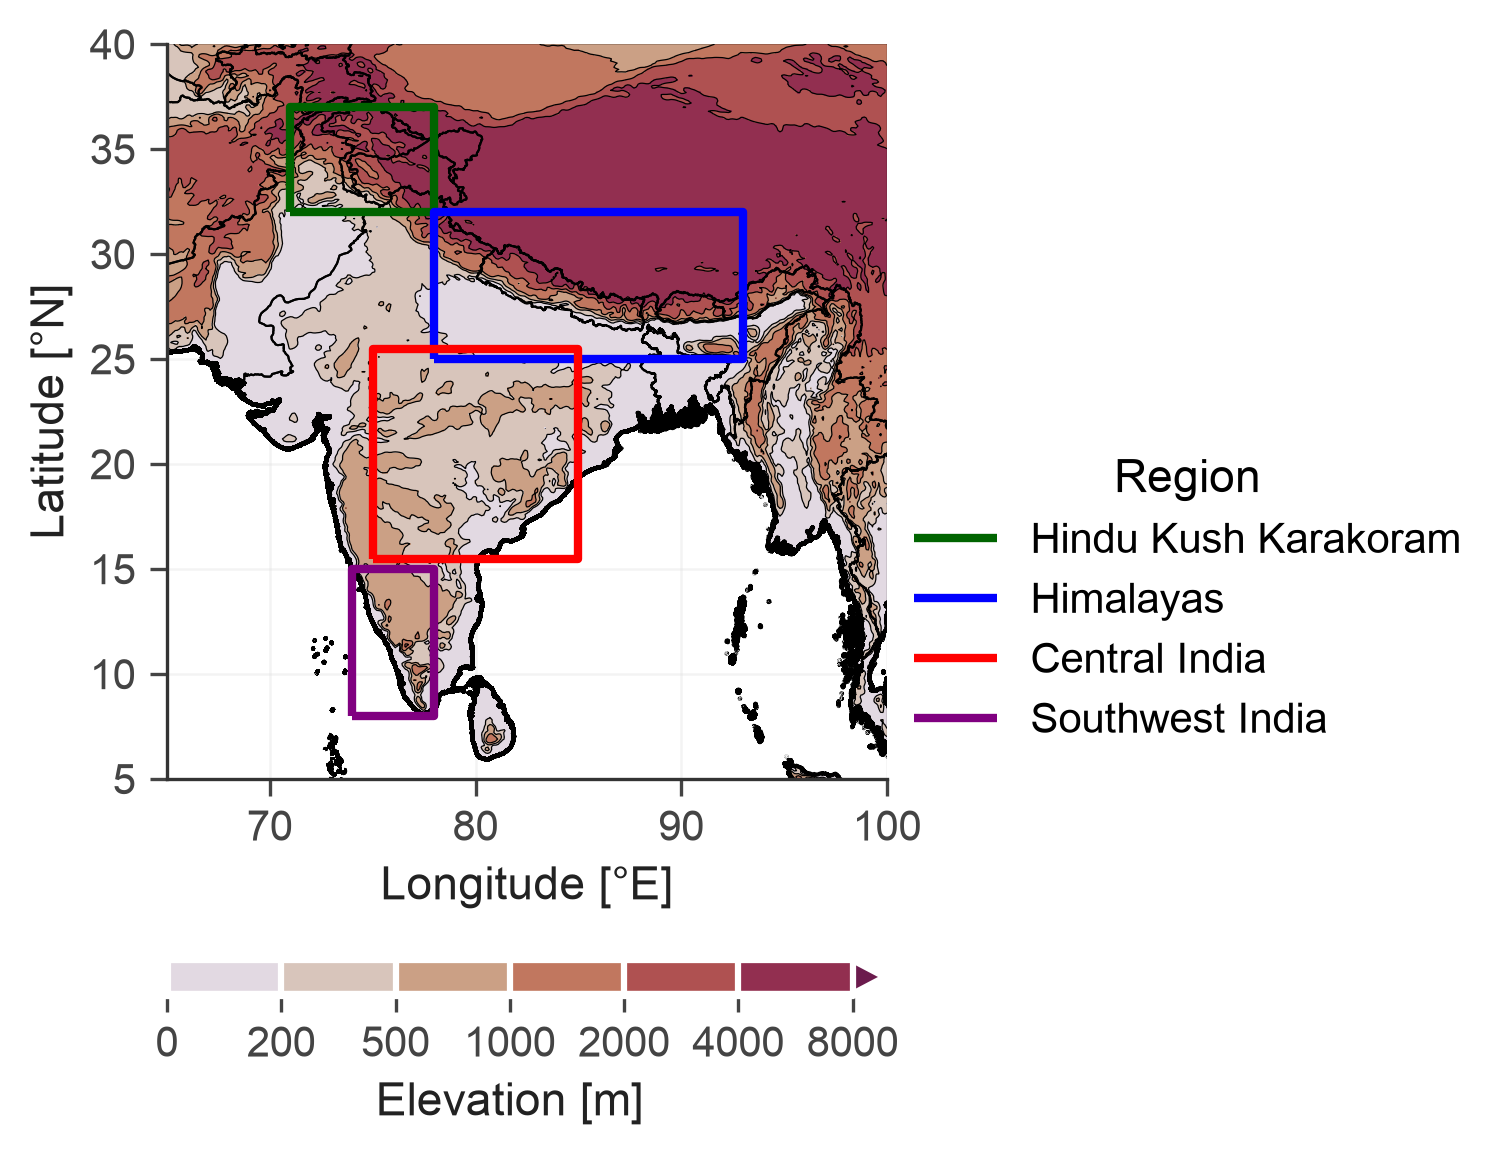
\includegraphics[width=0.75\linewidth]{Chapter3//figs/ERA5_orography_INDIA.png}
    \caption{Overview of the selected domain over the Indian subcontinent. 
    Orography is represented by shadings. 
    The four analyzed regions are highlighted by colored boxes.}
    \label{fig:india_orography}
\end{figure}

This climatic diversity makes the Indian subcontinent more than an illustrative application. In Central and Southwest India, the strong monsoon signal provides a relatively clear benchmark for evaluating whether the algorithm can identify established seasonal transitions. The Himalayan and Hindu Kush--Karakoram regions provide a more demanding test because of their complex topography and the interaction between summer and winter circulation systems. The case study therefore allows the framework to be evaluated under contrasting climatic conditions and makes it possible to assess whether a seasonal representation learned from climate data can be generalized without losing its physical meaning.

From a Climate Services perspective, the region also illustrates why seasonal information matters. Changes in monsoon onset or withdrawal can alter the timing of agricultural activities and water availability, while changes in the duration of winter can affect snowfall accumulation and downstream hydrology. A consistent method for identifying and tracking these seasonal phases can therefore transform multivariate climate data into indicators that are easier to compare across regions, models, and future periods.

\section{Data and Methods}

\subsection{Data}
We used both reanalysis and climate model simulations.
As reference, we employed ERA5 reanalysis daily data \citep{hersbach_era5_2020}, obtained from hourly outputs at original resolution (0.25° × 0.25°).
The variables considered are 2-meter temperature (tas), total precipitation (pr), and the zonal (ua850) and meridional (va850) wind components at 850 hPa.
These variables are among the most widely used in climatic characterization studies, as they jointly capture the main thermodynamic and dynamic components of the seasonal cycle. 

Reference values for the resulting seasonal transitions were compared with the most recent climatological normal onset and withdrawal dates of the Indian Summer Monsoon (ISM), as provided by the India Meteorological Department (IMD). The climatological normals correspond to the mean onset and withdrawal dates calculated over the period 1961–2019. These reference dates, available on a location-wise basis in \citet{pai_normal_2020}, were interpolated onto a 1° × 1° latitude–longitude grid using bilinear interpolation. The IMD dates are derived from a multi-step deterministic algorithm that combines precipitation thresholds with temporal continuity criteria. For a detailed description of this procedure, readers are referred to \citet{pai_normal_2020}.

To assess future changes, we analyzed a Coupled Model Intercomparison Project Phase 6 (CMIP6) Multi-Model Ensemble (MME), including both historical simulations (1961--2014) \citep{eyring_overview_2016} and future projections under the high-emission SSP5-8.5 scenario (2015--2100) \citep{oneill_scenario_2016}, using daily data. The ensemble includes one member for each different model to maximize model spread. 
The list of models used is reported in Table~\ref{tab:cmip6_models}.  

ERA5 and CMIP6 data underwent a common pre-processing pipeline.
First, all instances of 29\textsuperscript{th} February were removed to ensure a uniform 365-day calendar.
The data were then regridded to a common 1°~$\times$~1° latitude–longitude grid using bilinear interpolation to ensure spatial consistency across different native resolutions.
Finally, a 15-day centered rolling mean was applied to each variable to smooth high-frequency fluctuations and emphasize intra-seasonal variability relevant to the identification of meteorological seasons.

Since one of the goals of the analysis is to evaluate how seasonal patterns are represented in future projections, we additionally applied a common detrending and normalization procedure to both ERA5 and CMIP6 data in order to remove signals that could bias the detection. Specifically, for each variable and each grid point, standardized anomalies (z-scores) were computed within a 10-year moving window for every calendar day by subtracting the running mean and dividing by the corresponding running standard deviation. This normalization was therefore applied consistently across variables, spatial locations, and temporal windows in both datasets. The resulting standardized fields filter out low-frequency drifts, such as the gradual warming signal, and act as an effective debiasing procedure across models and periods, ensuring that the clustering and classification focus on the internal seasonal dynamics rather than on systematic model biases or long-term trends.

\subsection{Machine-Learning Framework}

To identify meteorological seasons in the current climate, to validate the capabilities of the models to reproduce them and to estimate their future evolution we adopted a two-step approach.  
First, we defined the baseline seasons from a set of multiple atmospheric variables using ERA5 reanalysis by applying an unsupervised temporal clustering algorithm.  
Second, we used a supervised classification model to extend this seasonal segmentation to the CMIP6 multi-model ensemble, both in present-day conditions and in future projections.  

In the first step, Radially Constrained Clustering (RCC; \citet{cannon_defining_2005}) was applied to identify temporally contiguous seasons.  
In the second step, a Multinomial Logistic Regression Classifier (MLRC; \citet{hastie_elements_2009}) was trained to learn the association between atmospheric states and the RCC-derived seasonal labels.  
Once trained, the MLRC was applied to classify each day in the CMIP6 MME.  
This framework allowed us to assess the ability of CMIP6 models to reproduce the seasonal cycle identified in ERA5 and to explore projected changes in seasonal characteristics over the 21\textsuperscript{st} century.

\subsubsection{Radially Constrained Clustering}
The Radially Constrained Clustering algorithm (RCC; \citet{cannon_defining_2005}) is used to define a number $k$ of seasons by their breakpoints $B=\{b_1, ... ,b_k\}$, i.e. the dates that mark the transition from one season to another.
In this study we set k = 4, corresponding to the four main phases of the  seasonal cycle in India : winter, pre-monsoon, monsoon, and post-monsoon. This choice was made to obtain a level of temporal granularity that is consistent with the commonly used seasonal description of the Indian climate and allows a direct comparison with existing literature and operational classifications. 

Differently with other widely used clustering algorithms that partition the data in the feature space (such as k-means \citep{lloyd_least_1982}), RCC ensures that the clusters are temporally disjoint. 
Furthermore, RCC treats the last day of the year as continuous to the first, allowing a season to span across the boundary between December $31^{st}$ and January $1^{st}$.

To run the clustering we considered, for each grid point, the four time series of tas, pr, ua850, and va850 from ERA5 for 59 years from 1961 to 2019. The temporal domain was chosen to align with the study by \citet{pai_normal_2020}, which defines the monsoon onset and withdrawal normal dates (i.e., the average onset and withdrawal date over the period 1961--2019). These dates were used as a reference for validating the results of the clustering in the present study. 

We reshaped the data into a design matrix $X$ with dimensions $365 \times 236$. Rows correspond to calendar days, while columns correspond to variable–year combinations. Since four variables (tas, pr, ua850, and va850) were considered over 59 years (1961--2019), the total number of features is $4 \times 59 = 236$. Thus, each column contains the 365--day annual cycle of one variable for one specific year. We then applied a min–max normalization independently to each feature to preserve the seasonal evolution and relative phasing of the variable throughout the year.

The clusters were then defined by the set $B$ of the $k$ breakpoints that minimizes the Within Clusters Sum of Squares (WCSS):

\begin{linenomath*}
    \begin{equation}
        WCSS = \sum_{i=1}^k \sum_{j \in c_i} \sum_{d \in D} \left( x_{j,d} - \mu_{i,d} \right)^2
    \end{equation}
\end{linenomath*}

where $x_{j,d}$ is the value of the feature $d \in D$ on day $j$, and $\mu_{i,d}$ is the mean value of feature $d$ within cluster $c_i$.

The minimum of the WCSS is searched through an iterative algorithm: 

\begin{enumerate}
    \item Generate a set $B$ of $k$ breakpoints equally spaced in the year.
    \item Update each breakpoint $b_i$ in $B$ by adding a random value drawn from $U(-\eta,\eta)$. In this work we set $\eta=3$.
    \item Compute WCSS over the design matrix $X$ using the updated breakpoints. 
    \item If WCSS decreases, retain the new breakpoints, otherwise, revert to the previous ones.
    \item Repeat steps 2-4 for a predefined number of iterations.
\end{enumerate}

\subsubsection{Multinomial Logistic Regression Classifier}

To project the seasons defined on ERA5 with RCC onto each climate model from CMIP6, we employed a Multinomial Logistic Regression Classifier (MLRC; \citet{hastie_elements_2009}). 
For each day, the MLRC estimates the probability of belonging to each season $k \in \{1,\dots,K\}$ using the SoftMax function:

\begin{linenomath*}
    \begin{equation}
        p_{i,k} = \frac{\exp(\mathbf{w}_k\cdot\mathbf{x}_i)}{\sum_{j=1}^{K} \exp(\mathbf{w}_j\cdot\mathbf{x}_i)}
    \end{equation}
\end{linenomath*}

where $\mathbf{x}_i$ is the vector of predictors (precipitation, near-surface air temperature, and zonal and meridional wind components), $\mathbf{w}_k$ is the weight vector for class $k$, and $p_{i,k}$ is the estimated probability that day $i$ belongs to season $k$.

The model parameters $\mathbf{w}$ are optimized by minimizing the categorical cross-entropy loss over $N$ samples:

\begin{linenomath*}
    \begin{equation}
        L = -\frac{1}{N} \sum_{i=1}^{N} \sum_{k=1}^{K} y_{i,k} \, \log(p_{i,k})
    \end{equation}
\end{linenomath*}

where $y_{i,k}$ is a binary indicator equal to 1 if sample $i$ belongs to season $k$, and 0 otherwise. 
The optimization is performed over multiple epochs using the Adam algorithm \citep{kingma_adam_2017}.

We trained the MLRC on ERA5 daily data for the period 1961--2009, using the seasons identified by the RCC as categorical labels. An independent MLRC was trained at each grid point, and the resulting pointwise classifications and coefficients were subsequently aggregated over the four representative regions. As predictors, we used the same four atmospheric variables employed in the clustering step (tas, pr, ua850, va850), thus ensuring full consistency between the unsupervised and supervised phases of the framework.
As predictors, we used the same four atmospheric variables employed in the clustering step (tas, pr, ua850, va850) thus ensuring full consistency between the unsupervised and supervised phases of the framework.
The training dataset comprised 17,885 daily samples, which were divided into batches of size 52, and the model was trained over 100 epochs.

Since the MLRC is based on a linear decision function, the learned coefficients provide a direct interpretation of the influence of each predictor on the seasonal classification \cite{hastie_elements_2009}. To compare the relative role of the different predictors, we quantified their importance from the normalized magnitude of the class-specific coefficients:
\begin{equation}
I_{m,k} =
\frac{|w_{m,k}|}
{\sum_{m=1}^{M}|w_{m,k}|}
\times 100 (\%),
\end{equation}
where $w_{m,k}$ denotes the coefficient associated with predictor $m$ in the weight vector $\mathbf{w}_k$. By construction, the resulting importance values sum to 100\% for each season and grid point, providing an interpretable measure of the relative contribution of temperature, precipitation, zonal wind, and meridional wind to the classification.

\subsubsection{Validation and skill}

To assess the capability of the CMIP6 MME to reproduce the seasonal cycle and the effectiveness of our classification algorithm in identifying the correct season, we classified each day of each model for the period that overlaps ERA5 (1961-2015), and we computed the $F1$ Score \cite{blair_information_1979} for each model and season across the four spatial boxes (Figure \ref{fig:india_orography}). 

To provide an out-of-sample reference for classifier performance, the trained MLRCs were also applied to the held-out ERA5 period 2010--2019, and the resulting F1 scores were computed against the RCC-derived seasonal labels.


$F1$ score is the harmonic mean of precision and recall, and it is defined as:

\begin{linenomath*}
    \begin{equation}
        F1=2*\frac{precision*recall}{precision+recall}
    \end{equation}
\end{linenomath*}

where the precision measures the fraction of days classified in the season $x$ that actually belong to season $x$, and the recall the fraction of days classified in the season $x$ over the total number of days in the season $x$:

\begin{linenomath*}
    \begin{equation}
            precision = \frac{True\ positive}{True\ positive + False\ positive}\\
    \end{equation}
\end{linenomath*}

\begin{linenomath*}
    \begin{equation}
            recall = \frac{True\ positive}{True\ positive + False\ negative}
    \end{equation}
\end{linenomath*}

Values of $F1$ range from 0 to 1, with higher scores indicating better agreement between the predicted and reference seasonal labels. 
A value close to 1 denotes high classification accuracy, meaning that most days are correctly assigned to their corresponding season. 
In the present four-class problem, a random assignment would yield an expected $F1$ of approximately 0.25. 
Therefore, values around 0.5 indicate that the model performs roughly twice as well as random guessing, representing a threshold between poor and moderate skill. 
In this study, we adopt $F1 = 0.7$ as a practical threshold for good performance. 
From the definition in Eq. 4, this value implies that neither precision nor recall can fall below 0.5 unless the other is very high (e.g., $P = 0.9$ if $R = 0.5$). 
Hence, setting the threshold at 0.7 ensures that both metrics are simultaneously satisfactory, balancing detection capability and false alarm rate.

\section{Results}

\subsection{Meteorological Seasons from Reanalysis Data}

The first step of the framework consists of allowing the RCC algorithm to learn the meteorological seasons from ERA5 reanalysis data. We applied the algorithm to every grid point within the study domain and then aggregated the resulting seasonal breakpoints by averaging them over the four subregions shown in Figure~\ref{fig:india_orography}. We then assessed whether the seasonal partition identified by the RCC was consistent with the operational classification adopted by the IMD. The aim was to determine whether, beyond the mathematical consistency of the clustering, the resulting seasons corresponded to established operational definitions and could therefore provide meaningful information for real world applications.

We found that the clustering identifies four distinct seasons that closely reproduce the partitioning adopted by the IMD: monsoon (June--September), post-monsoon (October--November), winter (December--February), and pre-monsoon (March--May) \citep{praveen_analyzing_2020}, as shown in Figure~\ref{fig:clustering_results_polar}.  
The timing of monsoon onset and withdrawal aligns well with the IMD-defined phases of the Indian Summer Monsoon (ISM) \cite{pai_normal_2020}, with the onset in Southwest India (blue line) occurring earlier than in other regions, in agreement with the climatological progression of the monsoon (Figure~\ref{fig:clustering_results_polar}).  

For the other three seasons, whose boundaries are not as clearly defined in the literature, the clustering still provides a coherent segmentation (Figure~\ref{fig:clustering_results_polar}).  
The main discrepancy with the IMD subdivision emerges in the transition from winter to pre-monsoon, where the algorithm identifies a boundary that extends further into pre-monsoon.  
This behavior is more consistent with the definition of the Western Disturbance season proposed by \citet{palazzi_precipitation_2013}, spanning from December to April. Indeed the Hindu Kush-- Karakoram (yellow line) region is the one which present a longer winter season duration.  (Figure~\ref{fig:clustering_results_polar}). 

\begin{figure}[H]
    \centering
    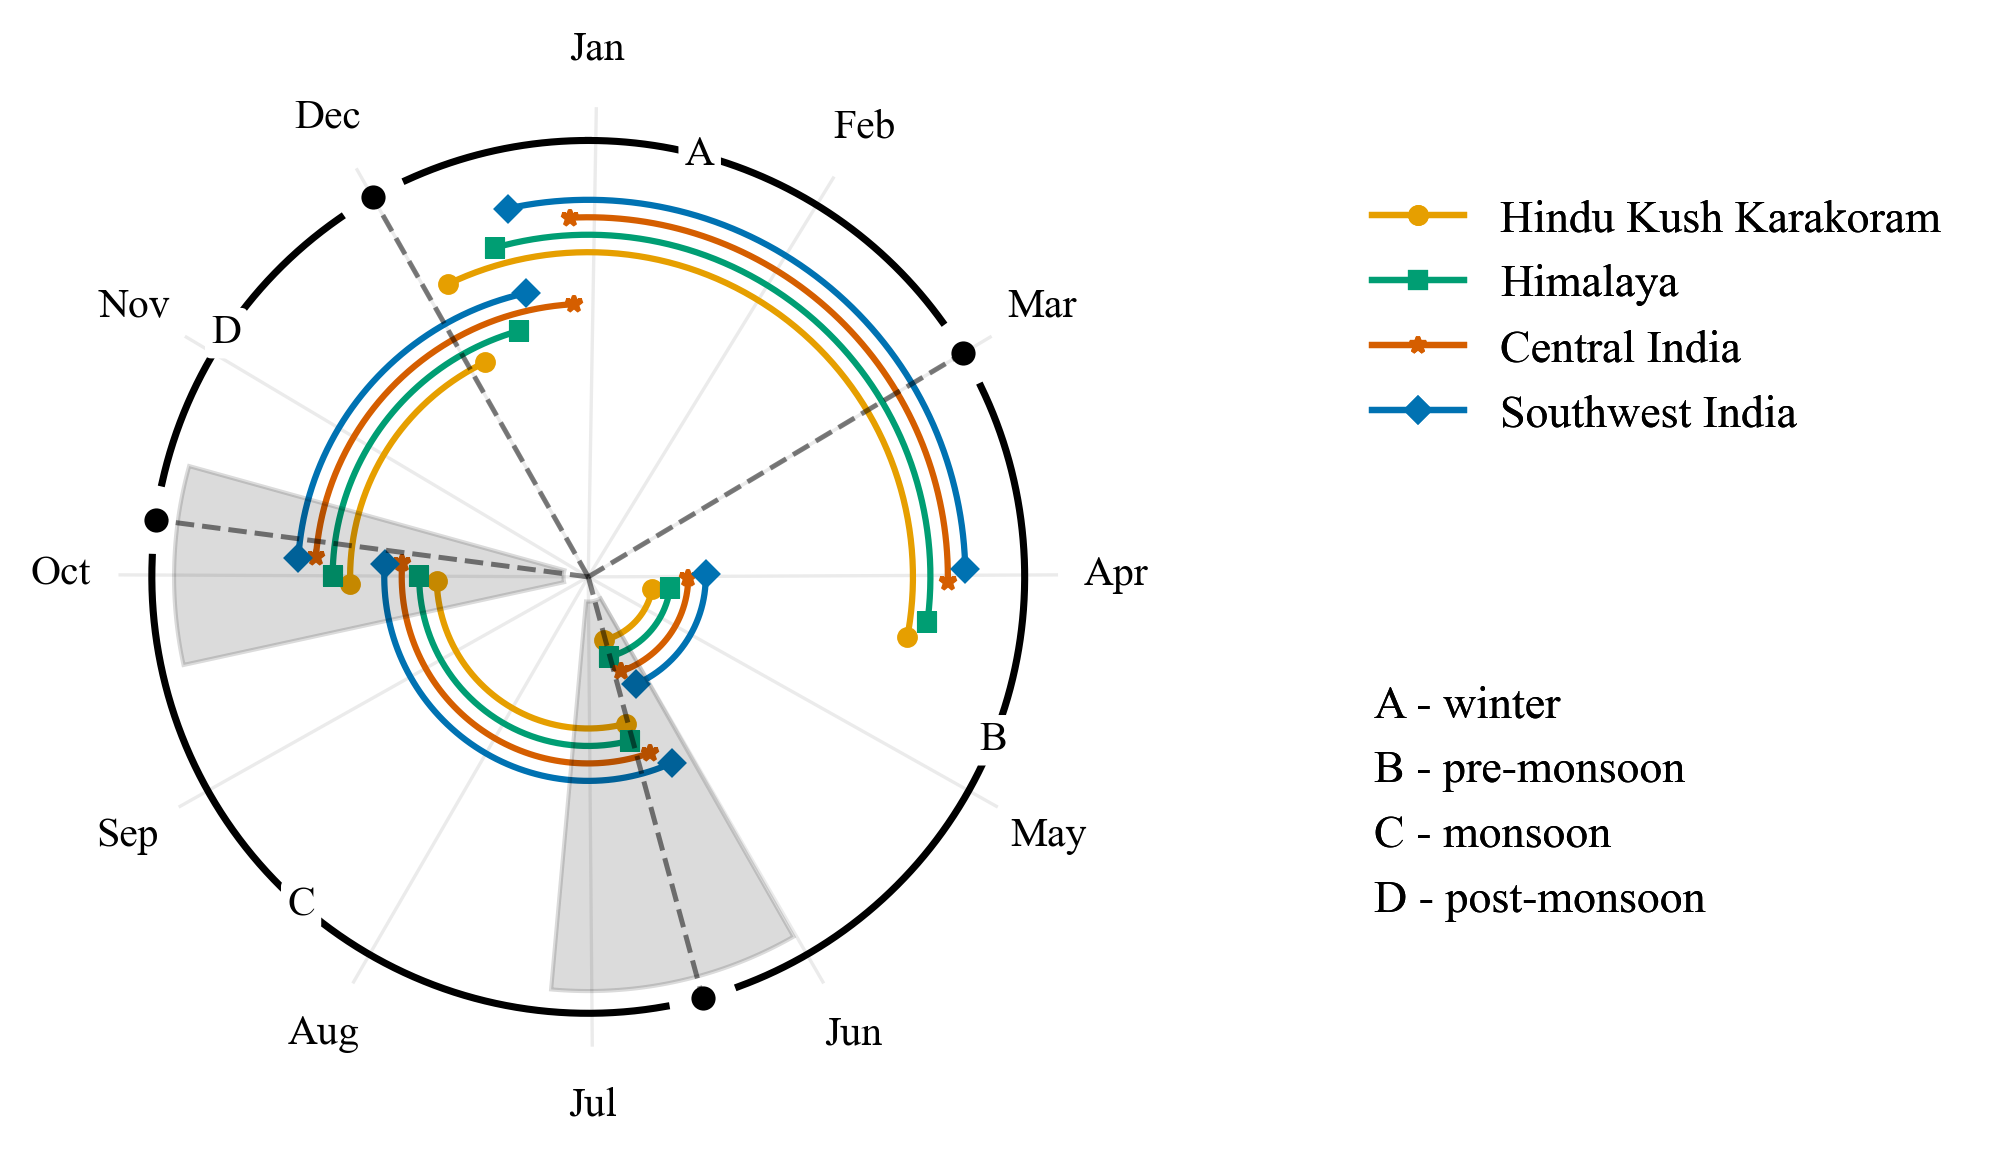
\includegraphics[width=0.8\textwidth]{Chapter3/figs/clustering_results_polar_coverage_all_regions.png}
        \caption{Seasonal coverage for the four focus regions. 
        Each colored arc corresponds to the median duration of the four identified seasons 
        (pre-monsoon, monsoon, post-monsoon, and winter), estimated from RCC clustering.
        The black outer reference ring highlights the subdivision adopted by the India Meteorological Department (IMD). 
        The shaded grey sectors around the monsoon onset and withdrawal represent the spatial variability (i.e., minimum and maximum dates) of IMD onset and withdrawal across India. 
        The monsoon onset and withdrawal medians are derived from \cite{pai_normal_2020}, using the normal onset and withdrawal dates averaged across the entire Indian landmass. 
        Month labels (e.g., ``Feb'') indicate the first day of each month, following a clockwise chronological order starting from January.}
        
    \label{fig:clustering_results_polar}
\end{figure}


Beyond the qualitative comparison, we also compared the identified breakpoints with the official monsoon onset and withdrawal normal dates provided by the IMD for each grid point over India. The RCC-derived monsoon onset is broadly consistent with the IMD climatology, although non-negligible regional differences are present. Positive differences occur in the southeastern part of the domain, corresponding to Andhra Pradesh, and in the northern part, corresponding to Ladakh, whereas negative differences are found in the northwestern part, particularly over Punjab and Rajasthan (see Figure \ref{fig:clustering_bias}a). 
A point-wise comparison of onset dates (Figure \ref{fig:clustering_dispersion}a) indicates that RCC tends to anticipate the advance of the monsoon relative to the IMD normals. 
The linear fit between the IMD reference dates (x-axis) and the RCC-derived dates (y-axis) yields a slope m=0.39, indicating that the spatial progression detected by RCC is more compressed in time than in the IMD reference. 
The spatial correspondence between the two fields is moderate, with a Pearson correlation coefficient r=0.35.

For monsoon withdrawal, the RCC--IMD differences are overall slightly positive, except over the southwestern part of the peninsula, where RCC identifies an earlier transition (Figure \ref{fig:clustering_bias}b). 
The point-wise comparison (Figure \ref{fig:clustering_dispersion}b) shows that RCC defines a slightly faster withdrawal progression (m=0.77), largely driven by the negative differences over the southern peninsula. The spatial correspondence is higher than for onset, with r=0.53. 
This result should nevertheless be interpreted cautiously, since the monsoon withdrawal has been less explored than the onset \citet{pai_normal_2020}, and its assessment remains challenging because of the larger interannual variability \citet{syroka_withdrawal_2004}.

\begin{figure}[H]
    \centering
    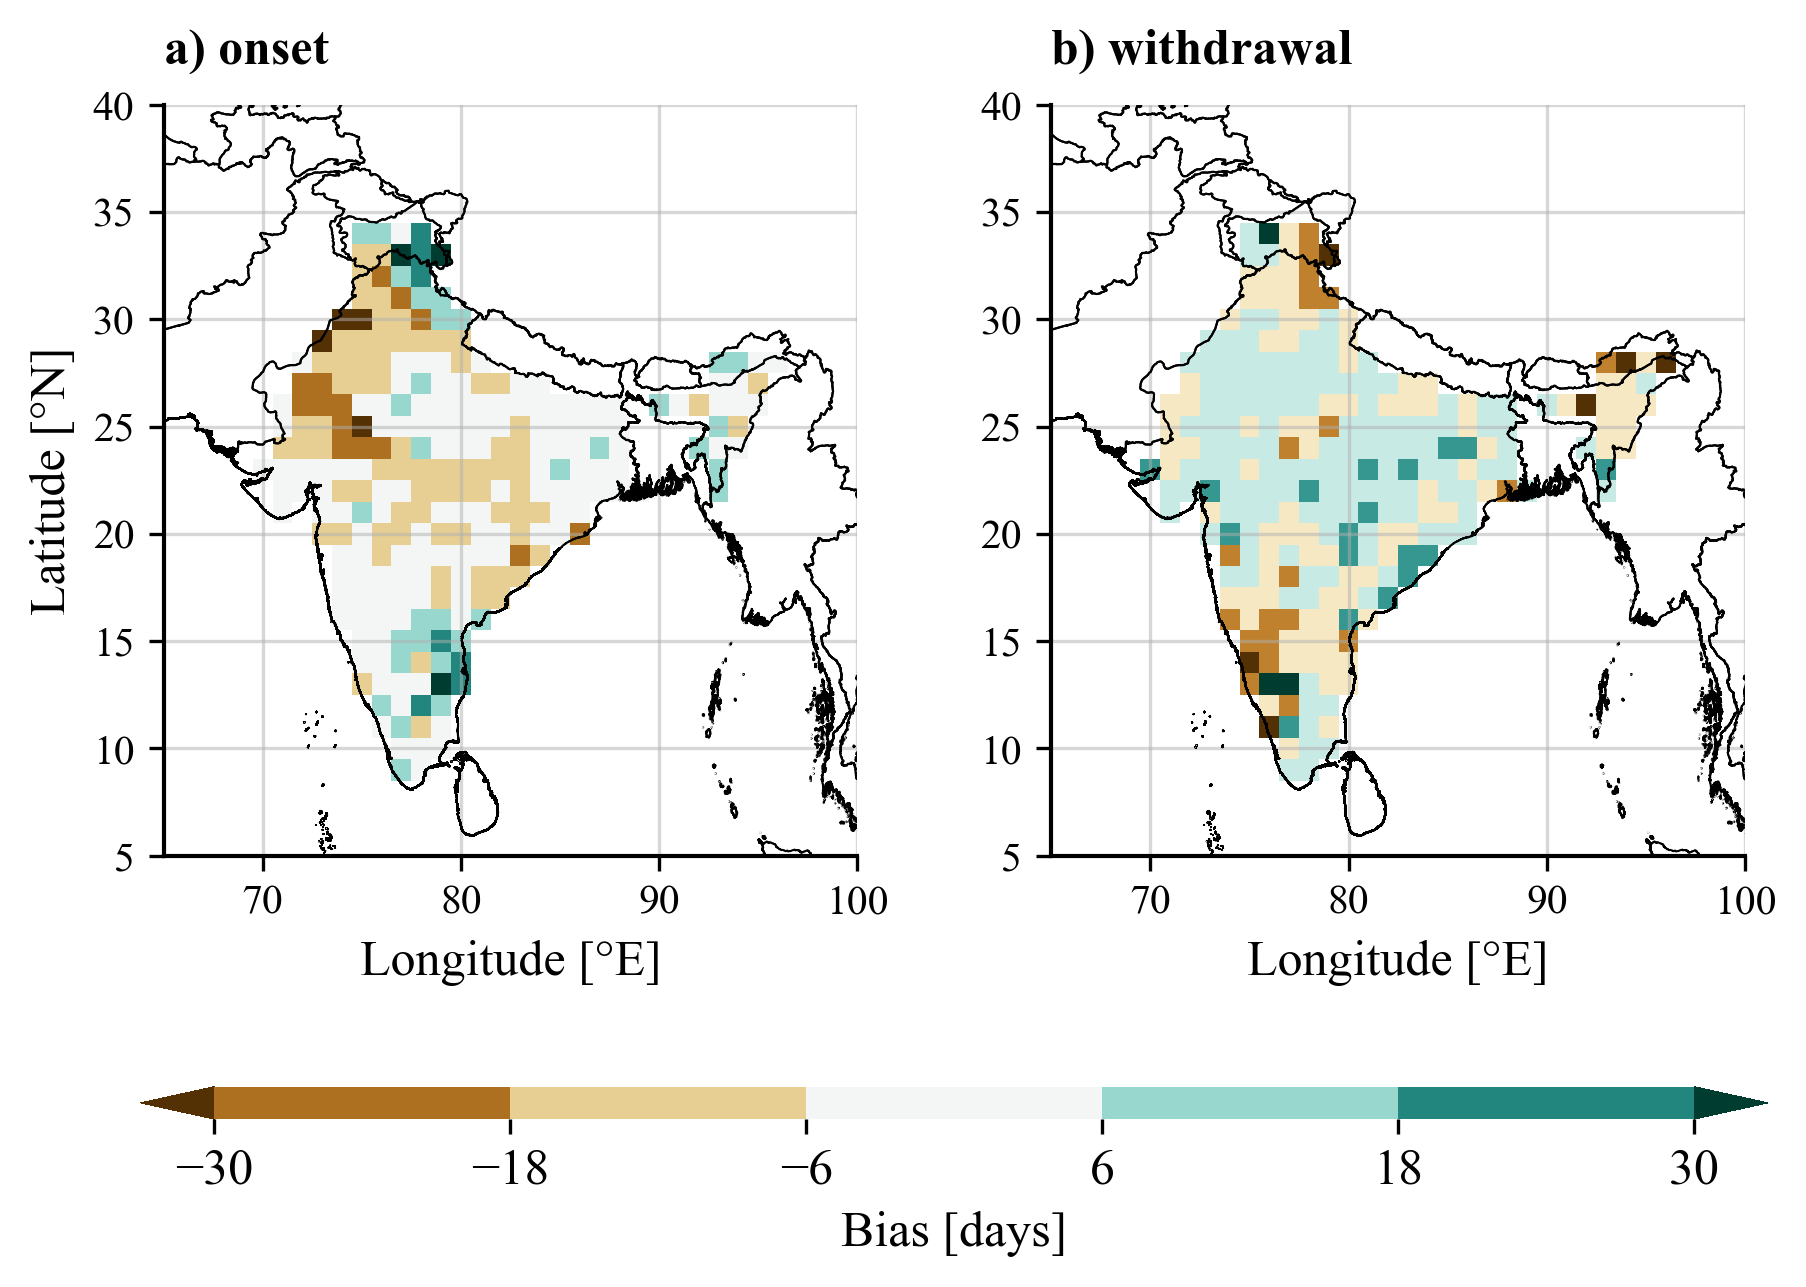
\includegraphics[width=0.7\textwidth]{Chapter3/figs/clustering_bias.png}
    \caption{Differences between the ISM phases by the RCC algorithm, compared to the reference dates provided by the IMD. Panel a shows the difference in monsoon onset dates between the RCC output and the IMD-defined climatological onset, while Panel b shows the difference in withdrawal dates. Positive values indicate a later transition identified by the RCC, and negative values an earlier one. Both fields are clipped over the IMD reference domain.}
    \label{fig:clustering_bias}
\end{figure}

\begin{figure}[H]
    \centering
    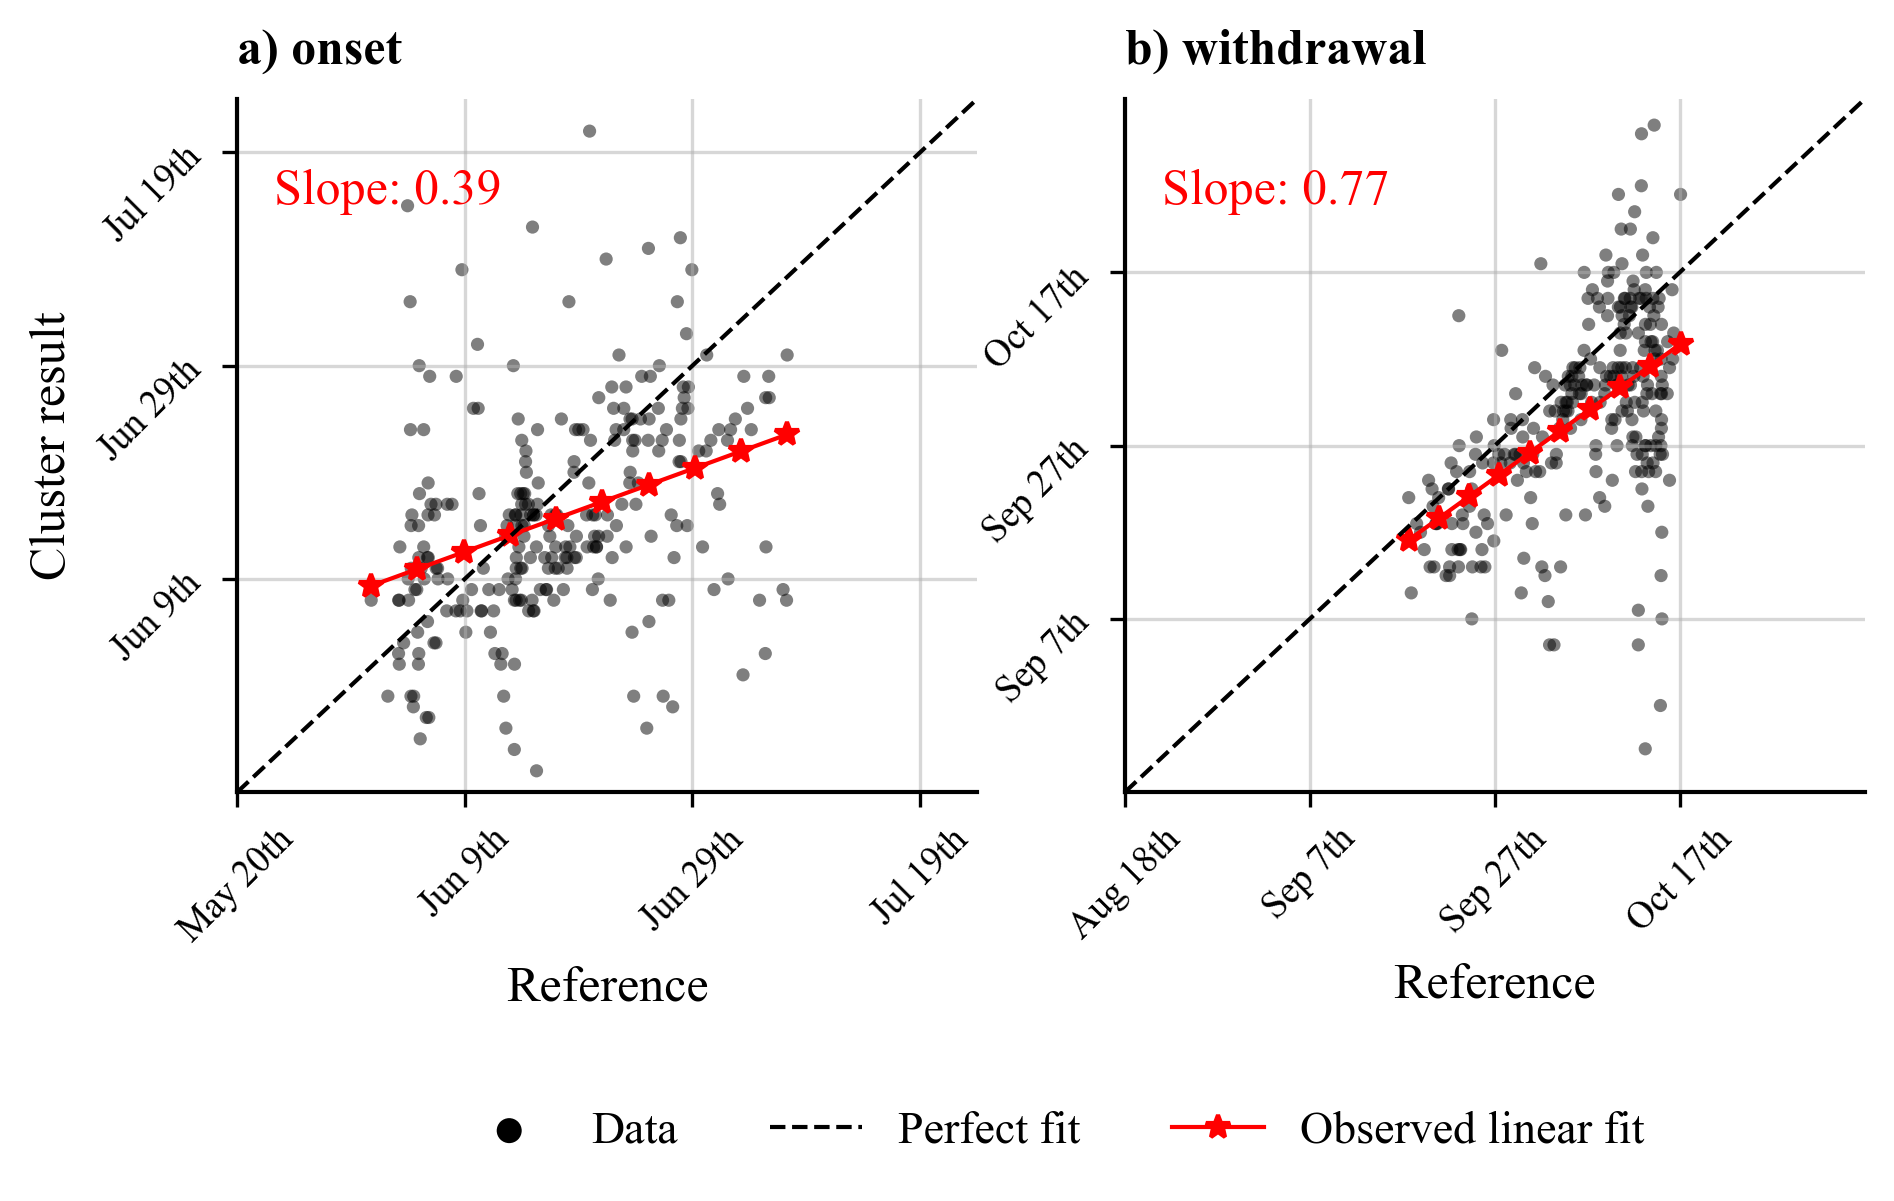
\includegraphics[width=0.7\textwidth]{Chapter3/figs/clustering_dispersion.png}
    \caption{Scatter plots comparing the seasonal transition dates identified by the RCC algorithm with the climatological reference dates from the IMD, across all grid points over the Indian subcontinent. Panel A shows the comparison for the monsoon onset, while Panel B refers to the monsoon withdrawal. Each point represents a single grid cell, with the reference date on the x-axis and the corresponding RCC-based date on the y-axis. The black dashed line indicates perfect agreement (1:1 line), while the red dashed line shows the linear regression fit. The slope of the fit is reported in each panel: slope weaker than 1 implies that the onset/withdraw of the monsoon system is progressing in space at a faster pace than in the IMD dataset.}
    \label{fig:clustering_dispersion}
\end{figure}

These discrepancies are expected given the different methodologies and data employed in defining and detecting monsoon transitions.
They reflect both dataset dependence and the fact that the two approaches diagnose related, but not identical, quantities.
IMD uses different criteria and data from multiple sources for defining the onset and withdrawal of the monsoon, while the RCC method identifies transitions between multivariate seasonal regimes using temperature, precipitation, and 850 hPa winds from ERA5 reanalysis only.
Accordingly, the RCC breakpoints should be interpreted as the onset and decay of a multivariate monsoon-like regime, rather than as precipitation-only onset or withdrawal dates.
Furthermore, while some studies have attempted to evaluate the reliability of ERA5 in reproducing regional precipitation patterns \citep{paul_spatial_2024, singh_assessment_2021}, the present comparison should not be read as an assessment of the ability of ERA5 to reproduce IMD transition dates, but as a benchmark of consistency for the multivariate seasonal segmentation.

Also considering these difference between approaches, it is clear that the RCC is able to produce a meaningful representation of the seasonal partition. In the next sections we will explore how this partition can be transferred to CMIP6 models, allowing an evaluation of the future expected changes.  

\subsection{Physical Intepretation}
Before applying the trained MLRC to the CMIP6 ensemble, we analyzed the relative importance of the model predictors in order to provide an interpretation of the classification framework. Using the normalized magnitude of the regression coefficients we quantified the contribution of temperature, precipitation, zonal wind, and meridional wind to the identification of each season. The resulting feature importance values are summarized in Table~\ref{tab:feature_importance}. The relative importance of the MLRC predictors varies substantially across seasons and regions.  Temperature is the dominant predictor during the pre-monsoon season in all four regions, accounting for 39--56\% of the total importance. Winter classification shows a stronger regional dependence, with temperature contributing most in HKK and the Himalaya (43--44\%), while precipitation becomes the leading predictor in Central and Southwest India (32--44\%). During the monsoon season, precipitation is the dominant predictor in the Himalaya and Central India (31--49\%), whereas zonal wind contributes most in Southwest India (39\%). Post-monsoon classification is characterized by a larger contribution from circulation-related variables, with zonal wind emerging as the dominant predictor in Central and Southwest India (36--40\%). Overall, the results indicate that the relative importance of the predictors is season- and region-dependent, with no single variable dominating the classification across all conditions.

\begin{table}[H]
\centering
\caption{Relative importance (\%) of the MLRC predictors. The dominant predictor for each season and region is shown in bold and underlined.}
\begin{tabular}{llcccc}
\hline
Season & Variable & HKK & Himalaya & Central India & Southwest India \\
\hline

winter
& tas   & \underline{\textbf{44}} & \underline{\textbf{43}} & 19 & 10 \\
& pr & 19 & 16 & \underline{\textbf{32}} & \underline{\textbf{44}} \\
& ua850          & 20 & 29 & 30 & 26 \\
& va850          & 17 & 13 & 19 & 21 \\
\hline

pre-monsoon
& tas   & \underline{\textbf{39}} & \underline{\textbf{42}} & \underline{\textbf{56}} & \underline{\textbf{45}} \\
& pr & 15 & 16 & 18 & 20 \\
& ua850          & 23 & 22 & 14 & 21 \\
& va850          & 23 & 20 & 13 & 14 \\
\hline

monsoon
& tas   & \underline{\textbf{38}} & 23 & 15 & 29 \\
& pr & 17 & \underline{\textbf{31}} & \underline{\textbf{49}} & 18 \\
& ua850          & 23 & 30 & 18 & \underline{\textbf{39}} \\
& va850          & 22 & 17 & 17 & 13 \\
\hline

post-monsoon
& tas   & \underline{\textbf{31}} & 15 & 30 & 29 \\
& pr & 30 & \underline{\textbf{36}} & 17 & 20 \\
& ua850          & 20 & 27 & \underline{\textbf{40}} & \underline{\textbf{36}} \\
& va850          & 19 & 22 & 14 & 14 \\
\hline

\end{tabular}
\label{tab:feature_importance}
\end{table}


\subsection{Transferring Seasonal Definitions to Climate Models}

The next step was to determine whether the seasonal definitions learned from ERA5 could be transferred meaningfully to climate model simulations. We therefore applied the trained MLRC to the historical simulations of the CMIP6 multi-model ensemble for the period 1961--2015. This evaluation is important because a statistically coherent definition derived from reanalysis data does not necessarily remain valid when applied to models characterized by different biases and representations of regional climate processes.

Figure~\ref{fig:f1_scores} summarizes the agreement between the ERA5-derived seasonal definitions and the classifications obtained from CMIP6. The figure also reports the performance of the classifier over the held-out ERA5 period 2010--2019. The ERA5 results provide a reference for interpreting the CMIP6 scores: when performance is high over ERA5 but lower over CMIP6, the difference is likely related to the representation of the seasonal cycle in the climate models. Conversely, low scores in both datasets suggest that the seasonal regimes themselves are less clearly distinguishable using the selected variables and classifier.

\begin{figure}[H]
\centering
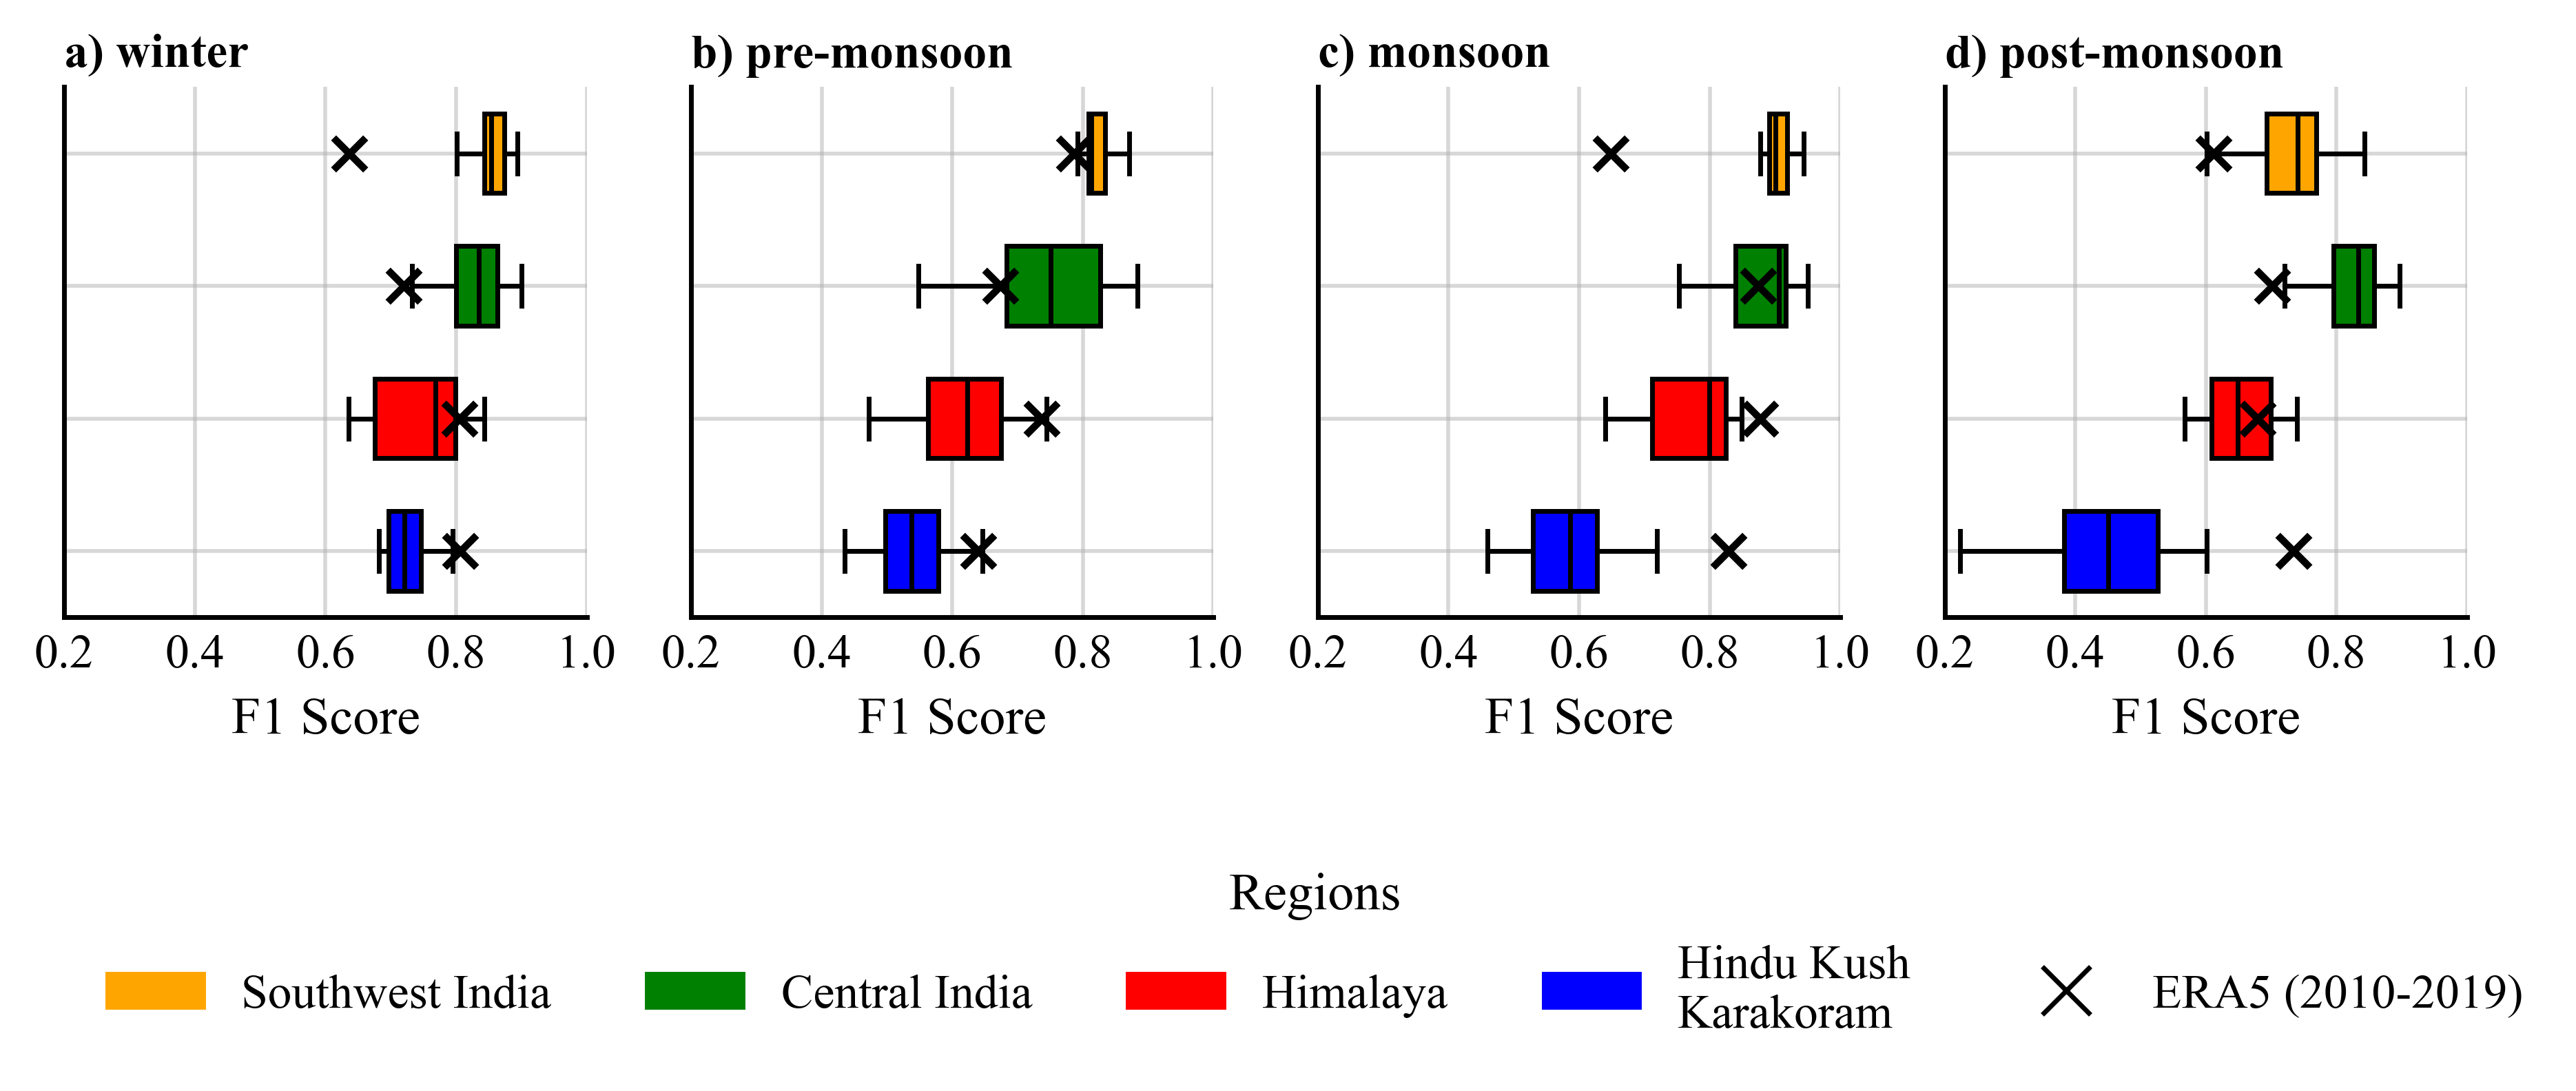
\includegraphics[width=0.9\textwidth]{Chapter3/figs/f1_scores.png}
\caption{Distribution of F1 scores computed for each season and CMIP6 model over the four representative regions during the historical period 1961--2015. The black crosses show the corresponding scores obtained over the held-out ERA5 period 2010--2019. Comparing CMIP6 with the ERA5 reference helps distinguish limitations of the classifier from differences in the seasonal cycle represented by the climate models.}
\label{fig:f1_scores}
\end{figure}

The seasonal cycle is represented consistently across the CMIP6 ensemble in Central and Southwest India. Performance is particularly strong for the monsoon, with average F1 scores of $0.86 \pm 0.09$ in Central India and $0.91 \pm 0.02$ in Southwest India. The monthly distribution of classified days confirms that the models reproduce both the overall shape and timing of the monsoon season, with only a small delay in its onset and close agreement in its withdrawal (Figure~\ref{fig:seasonal_shapes}c,d). Performance is slightly lower during the pre- and post-monsoon periods, whose transitional character makes their boundaries less clearly distinguishable.

\begin{figure}[H]
    \centering
    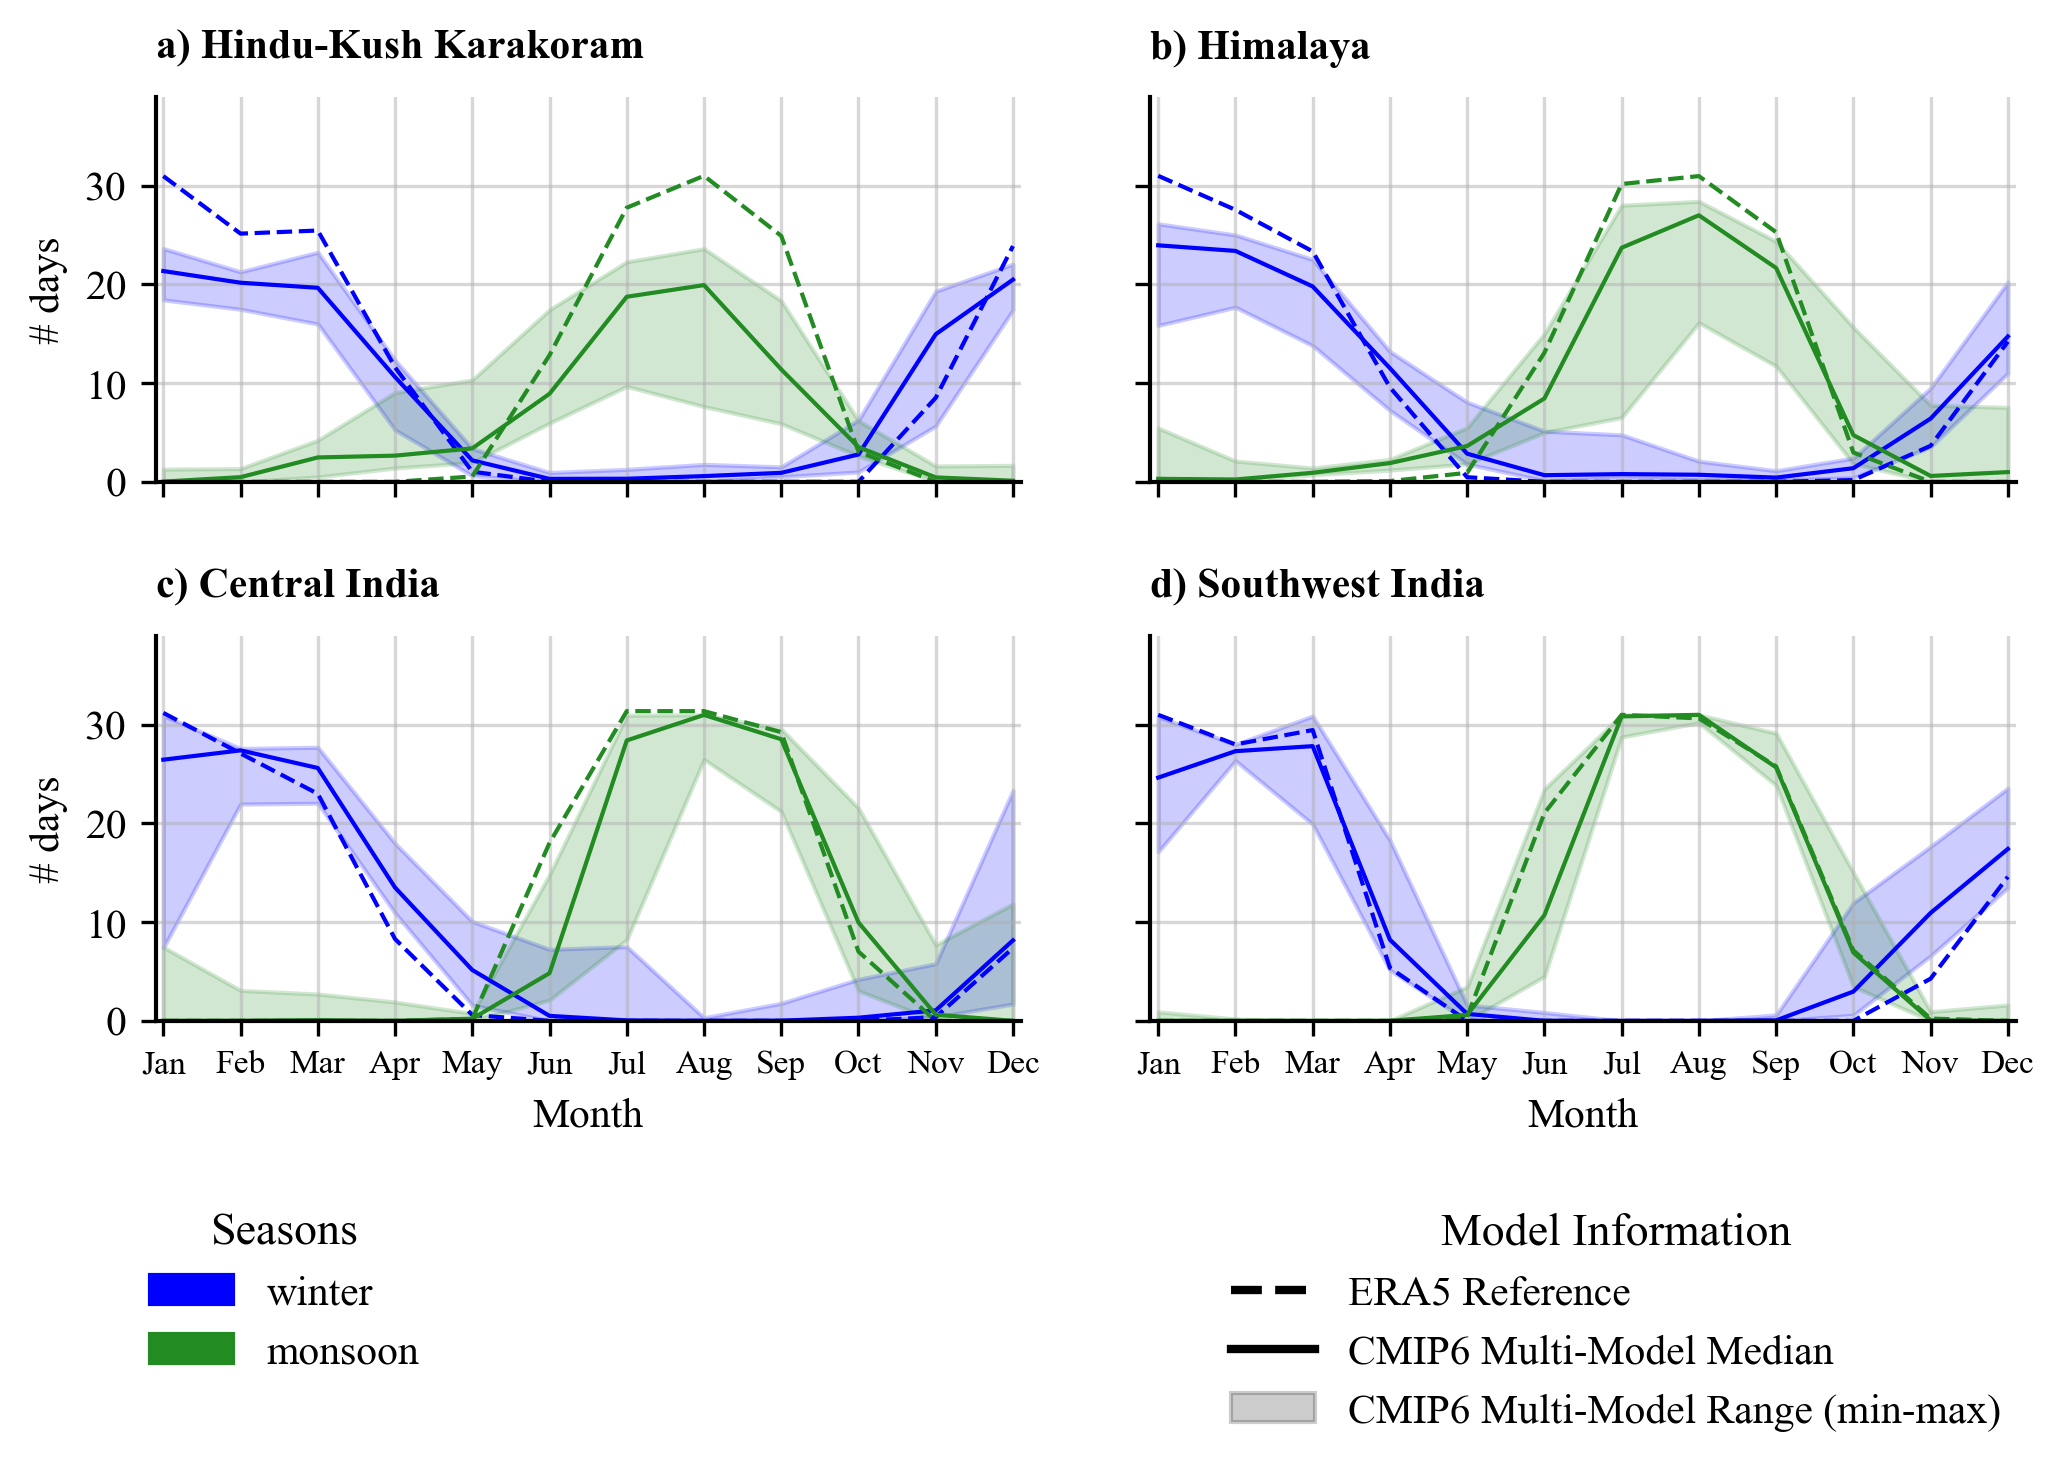
\includegraphics[width=0.9\textwidth]{Chapter3/figs/seasonal_shapes.png}
    \caption{Monthly distribution of days classified as winter and monsoon during the historical period over (a) Hindu Kush--Karakoram, (b) Himalaya, (c) Central India, and (d) Southwest India. Solid lines show the CMIP6 multi-model mean, shaded areas represent the inter-model range, and dashed lines show the seasonal classification derived from ERA5.}
    \label{fig:seasonal_shapes}
\end{figure}

The transfer is less successful in the mountain regions. Over the Hindu Kush--Karakoram, F1 scores are lower for the monsoon and transition seasons, with values ranging from $0.44$ for the post-monsoon to $0.56$ for the monsoon. The models reproduce the approximate timing of monsoon onset and withdrawal but classify fewer days as belonging to the monsoon during July and August (Figure~\ref{fig:seasonal_shapes}a). Because the corresponding ERA5 scores are generally higher, these differences appear to reflect primarily the difficulty of CMIP6 models in representing the regional seasonal cycle. The comparatively low ERA5 score during the pre-monsoon nevertheless indicates that this transition is also intrinsically more difficult to separate.

The Himalaya region shows intermediate performance, with F1 scores generally ranging between $0.6$ and $0.8$. The larger spread across models indicates that the representation of seasonality is less consistent than in Central and Southwest India. In both mountain regions, complex topography and the interaction between the summer monsoon and winter circulation make the seasonal cycle more difficult to reproduce. These results are consistent with the known ability of CMIP6 models to represent the main characteristics of the Indian monsoon \citep{khadka_evaluation_2022}, as well as with their limitations over the Himalayan region \citep{gusain_added_2020,lalande_climate_2021}.

The analysis shows that the seasonal definitions learned from reanalysis data can be transferred successfully to climate models where the underlying climatic regimes are represented with sufficient accuracy. At the same time, it demonstrates that the information obtained from the classification cannot be interpreted independently of model skill. For this reason, only models achieving an F1 score greater than $0.7$ for a given grid point and season were retained in the Significant Multi-Model Ensemble used for the analysis of future changes. This selection ensures that projected changes are evaluated only where the historical seasonal cycle is represented with adequate reliability.


\subsection{Projected Changes in Seasonality}

Having established where the ERA5-derived seasonal definitions can be transferred reliably to climate models, we applied the framework to future CMIP6 projections to investigate how the annual cycle may evolve during the twenty-first century. The analysis focuses primarily on the monsoon and winter seasons, which exhibit the clearest climatic signals and the greatest societal relevance. 

For each grid point and season, we retained only the models with an historical F1 score greater than $0.7$. This subset, referred to as the Significant Multi-Model Ensemble (SMME), accounts for the regional differences in the ability of CMIP6 models to reproduce the observed seasonal cycle. As summarized in Table~\ref{tab:smme_median_percentage}, nearly all models satisfy this criterion in Central and Southwest India, whereas considerably fewer models are retained over the Himalaya and Hindu Kush--Karakoram. Projected changes over the mountain regions should therefore be interpreted with greater caution.

\begin{table}[H]
\centering
\caption{Median number of models included in the Significant Multi-Model Ensemble for each season and region. Percentages refer to the complete ensemble of 13 models.}
\begin{tabular}{lcccc}
\hline
\textbf{Region} & \textbf{Winter} & \textbf{Pre-monsoon} & \textbf{Monsoon} & \textbf{Post-monsoon} \\
\hline
Hindu Kush--Karakoram & 8 (62\%) & 2 (15\%) & 6 (46\%) & 1 (8\%) \\
Himalaya              & 9 (69\%) & 6 (46\%) & 10 (77\%) & 7 (54\%) \\
Central India         & 12 (92\%) & 10 (77\%) & 12 (92\%) & 11 (85\%) \\
Southwest India       & 13 (100\%) & 12 (92\%) & 13 (100\%) & 12 (92\%) \\
\hline
\end{tabular}
\label{tab:smme_median_percentage}
\end{table}

Future changes were examined from three complementary perspectives. Figure~\ref{fig:spatial_trends} shows the spatial distribution of long-term trends in seasonal duration, while Figure~\ref{fig:seasonal_increment} describes their evolution within the four representative regions. The monthly analyses in Figures~\ref{fig:monthly_increment_monsoon} and \ref{fig:monthly_increment_winter} show which parts of each season contribute to the projected changes, allowing shifts in onset and withdrawal to be distinguished from uniform changes in duration.

\begin{figure}[H]
    \centering
    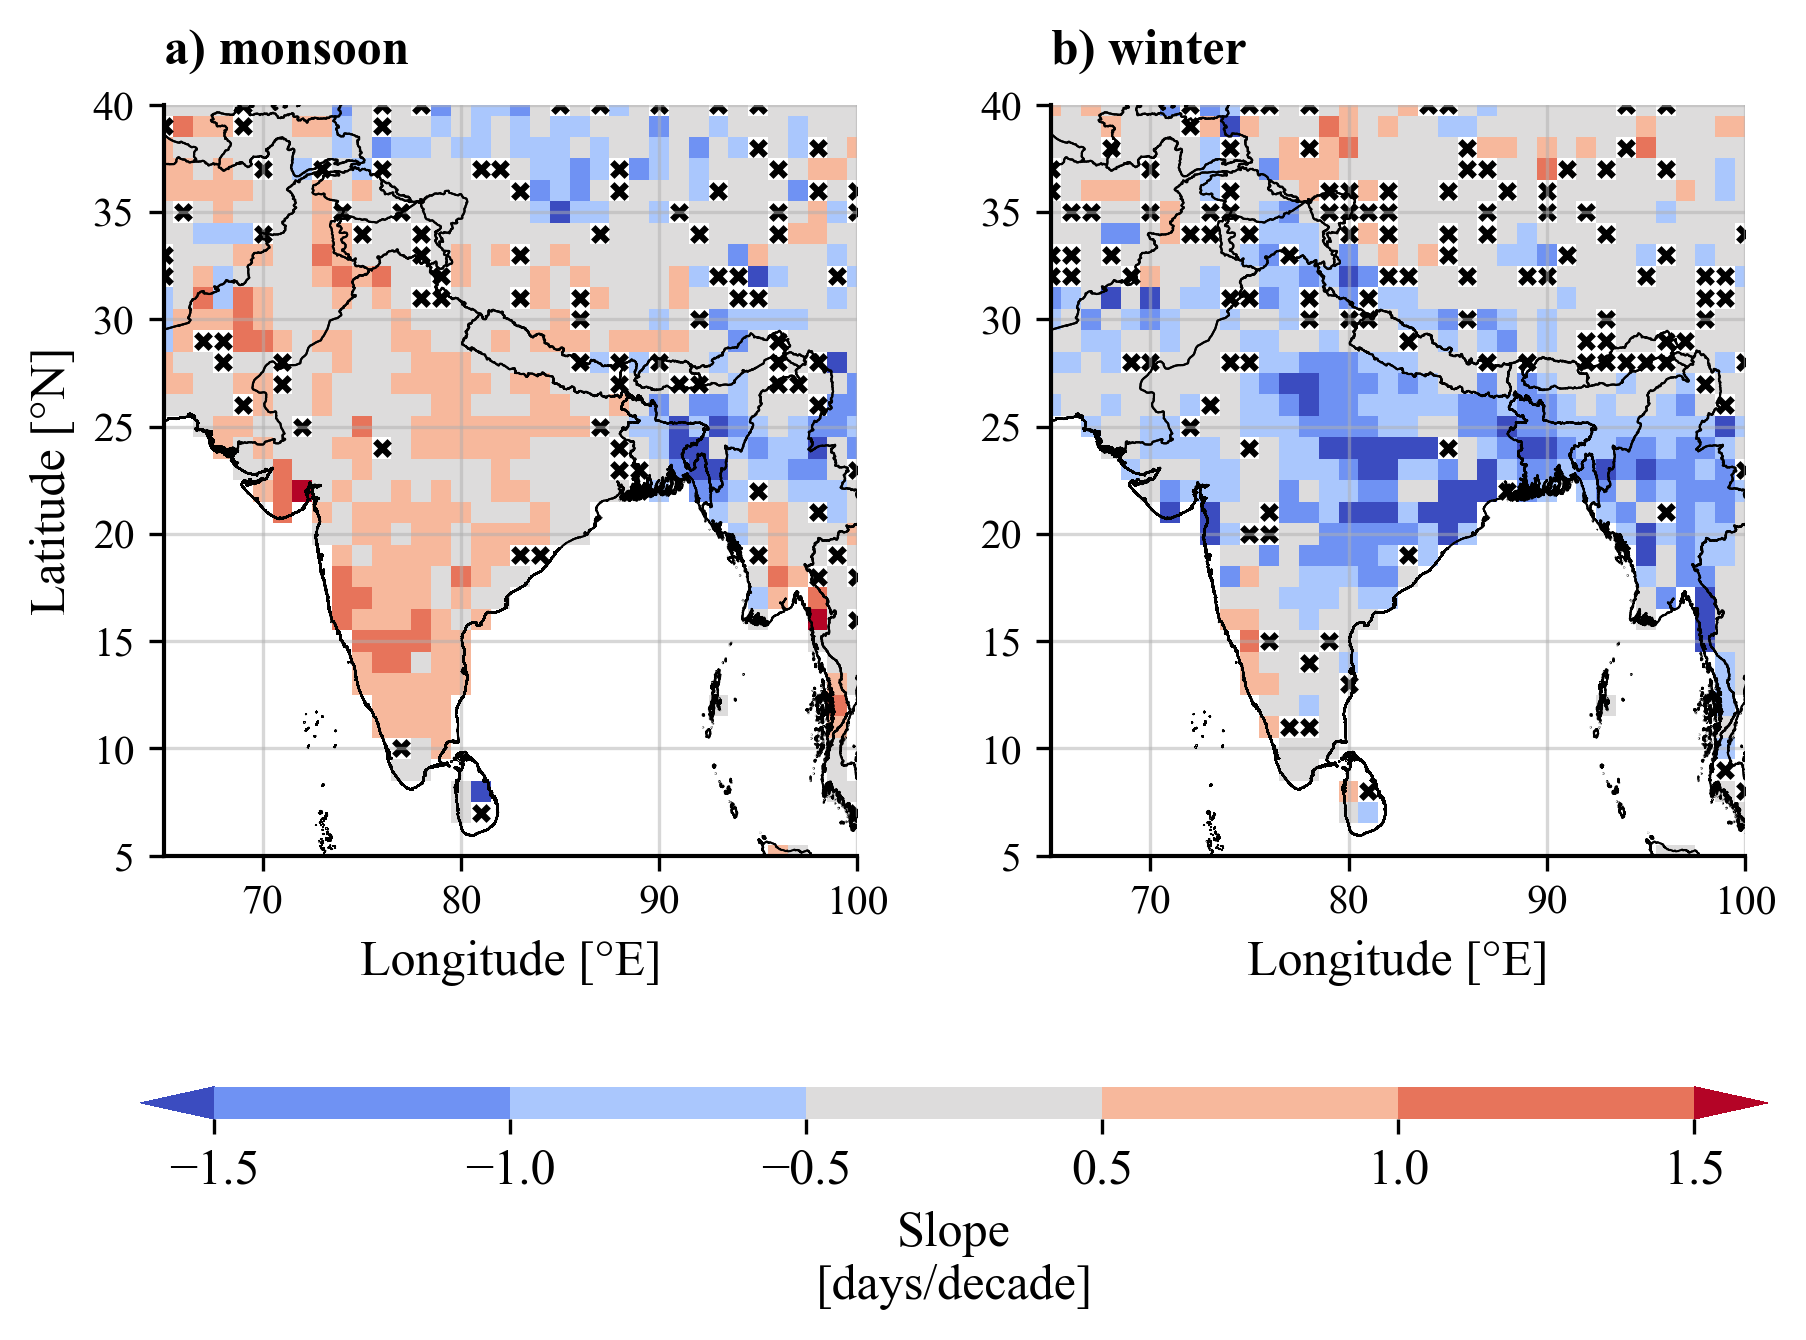
\includegraphics[width=0.7\textwidth]{Chapter3/figs/spatial_trends.png}
    \caption{Spatial distribution of linear trends in the number of days classified as monsoon (a) and winter (b) over the Indian subcontinent during 2020--2100. Trends are expressed in days per decade and computed from the SMME mean. Only trends significant at the 95\% confidence level according to the Mann--Kendall test are shown \citep{gilbert_statistical_1987}. Black crosses identify grid points without statistically significant trends.}
    \label{fig:spatial_trends}
\end{figure}

\begin{figure}[H]
    \centering
    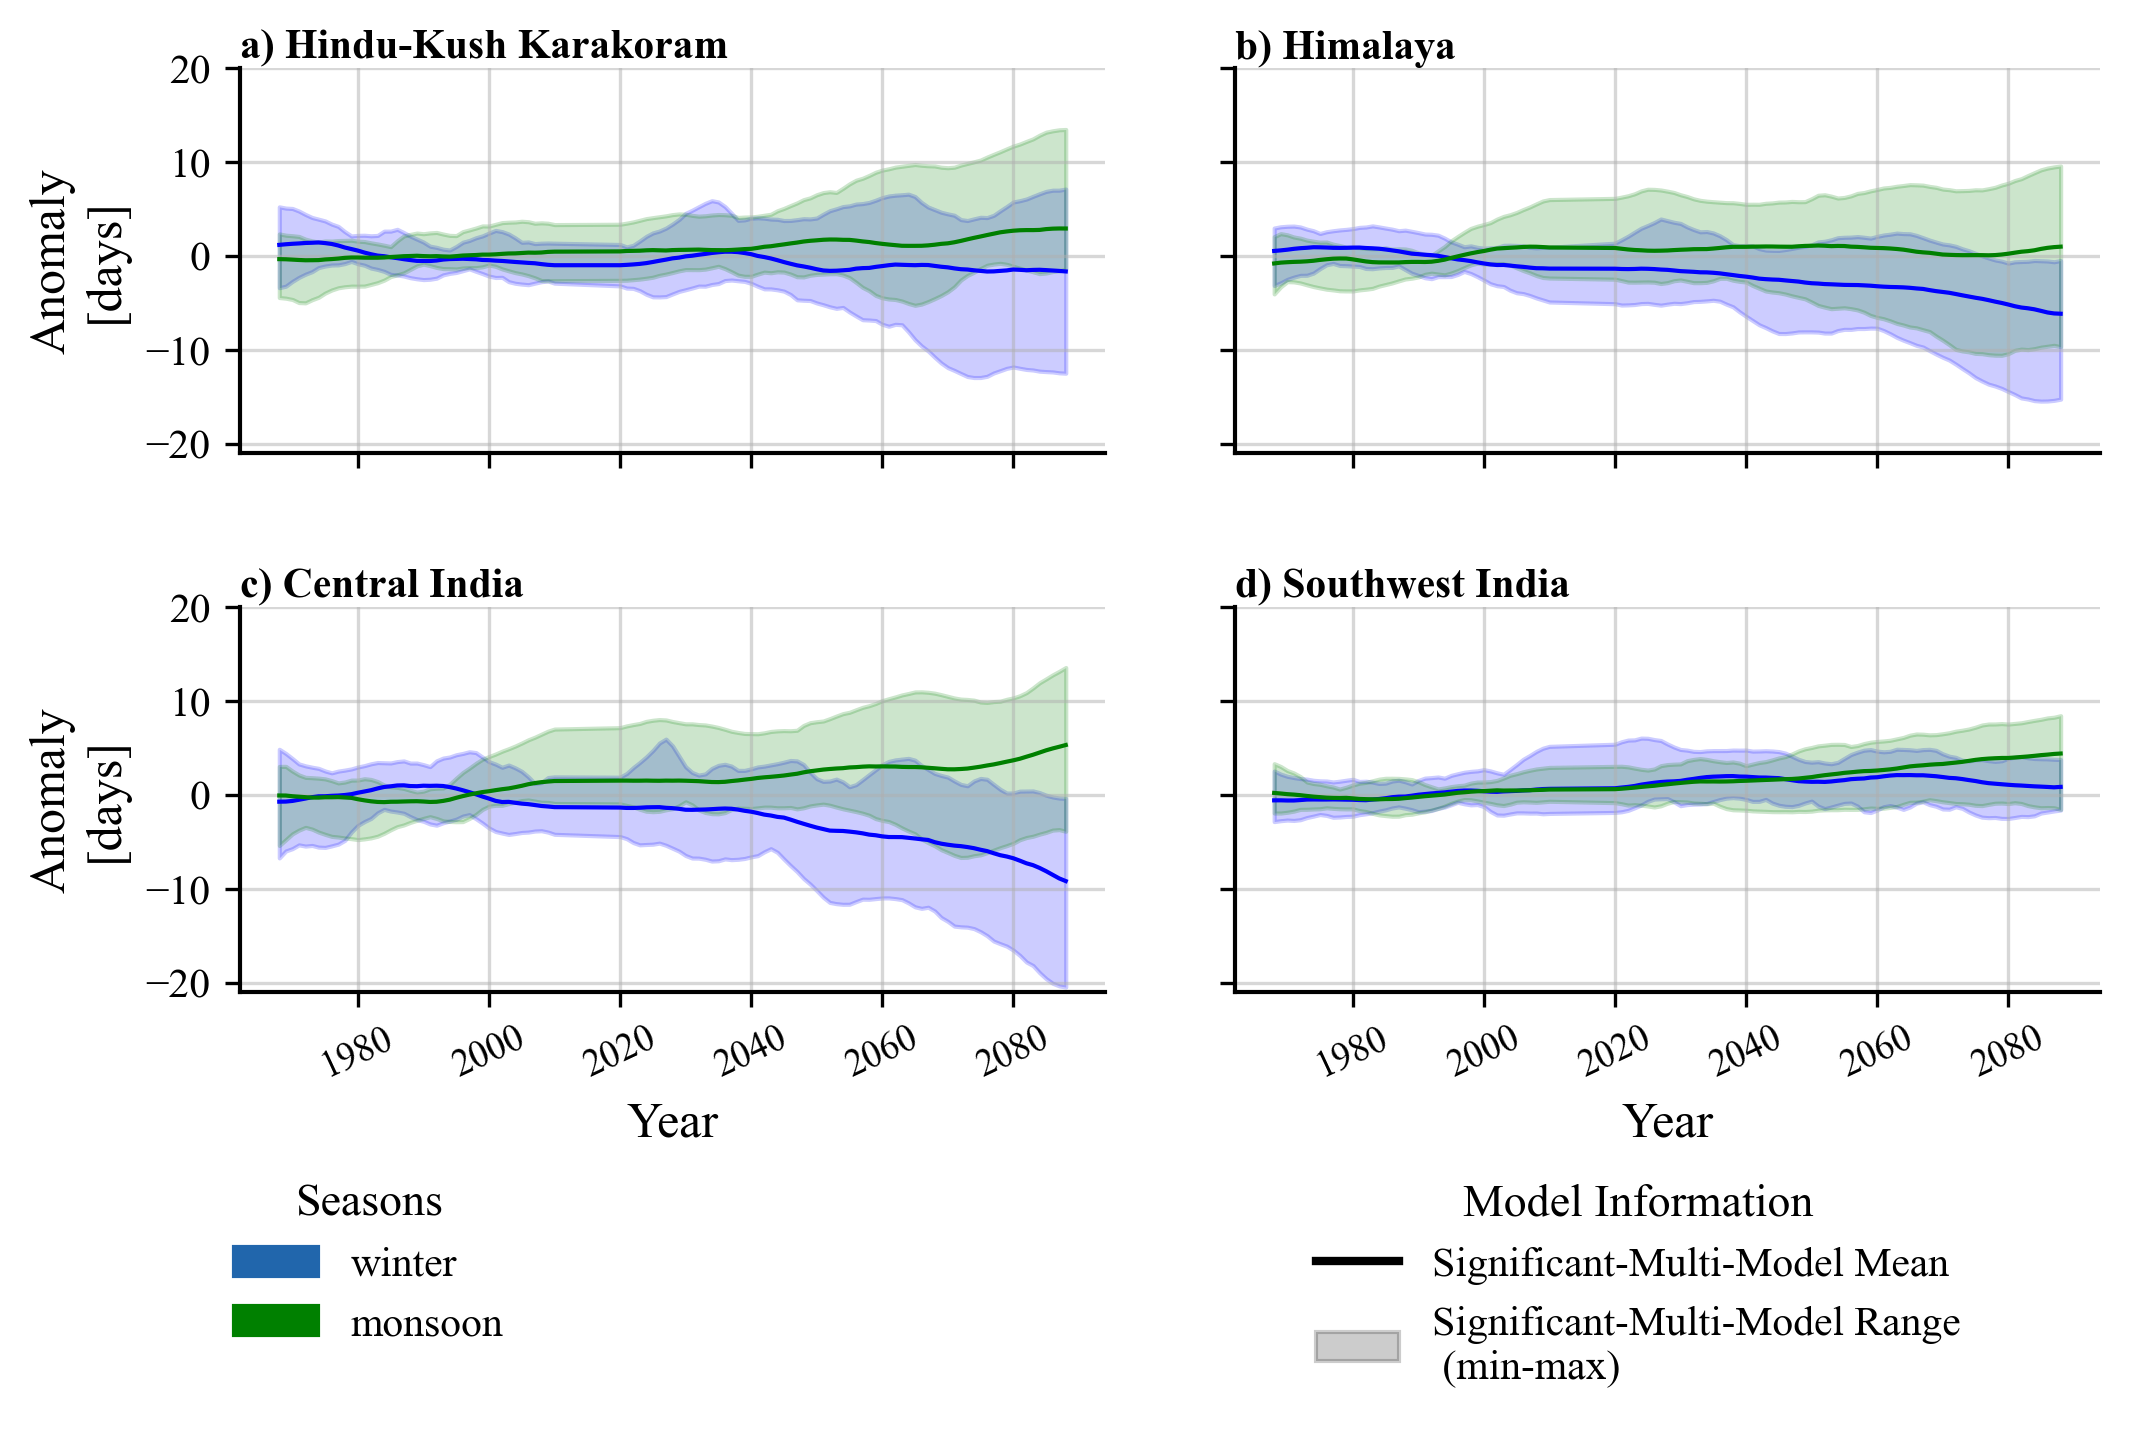
\includegraphics[width=0.9\textwidth]{Chapter3/figs/seasonal_increment.png}
    \caption{Projected anomalies in winter and monsoon duration over the four representative regions. Anomalies are computed relative to the historical mean seasonal length for 1970--2020 and smoothed using a 15-year centred rolling average. Solid lines represent the SMME mean and shaded areas show the inter-model range.}
    \label{fig:seasonal_increment}
\end{figure}

Most of the Indian subcontinent shows a significant lengthening of the monsoon season, particularly across Central, Western, and Southern India, where trends exceed $+0.5$ days per decade in several areas (Figure~\ref{fig:spatial_trends}a). Signals are weaker and less spatially coherent in northern and northeastern regions.

Central and Southwest India exhibit the clearest changes, with the monsoon projected to lengthen by approximately five days by the end of the century (Figure~\ref{fig:seasonal_increment}c,d). This extension is asymmetric: monsoon onset changes only slightly, while withdrawal occurs progressively later (Figure~\ref{fig:monthly_increment_monsoon}c,d). The result therefore indicates a persistence of monsoon-like conditions into the later part of the annual cycle rather than a uniform expansion at both seasonal boundaries.

The Himalayan region shows little change in total monsoon duration, but its internal timing shifts by approximately two days from the early to the late part of the season (Figure~\ref{fig:monthly_increment_monsoon}b). No consistent trend emerges over the Hindu Kush--Karakoram, where models produce a combination of weak positive and negative changes. The low historical skill and limited number of models retained in the SMME further reduce confidence in projections for this region.

These results are broadly consistent with CMIP6 studies projecting an increase in Indian monsoon precipitation, wet days, and heavy precipitation under global warming \citep{wang_understanding_2020,norgate_present_2024,dhara_post-ar6_2025}. Previous analyses based on precipitation thresholds have also identified a delayed withdrawal of the Indian Summer Monsoon \citep{ha_future_2020,wang_rainy_2002}. The present framework reaches a similar conclusion using a multivariate classification of the regional atmospheric state.

However, the direction of projected changes depends on how the monsoon is defined. Using a large-scale indicator based on the upper-tropospheric temperature gradient, \citet{cheng_shorter_2025} found a shortening of the monsoon under a high-emission scenario, characterized by delayed onset and earlier withdrawal. This apparent contrast reflects the fact that the two approaches describe different components of the monsoon system. The large-scale temperature gradient represents the establishment and decay of monsoon circulation, whereas the classification used here identifies the persistence of local hydroclimatic conditions. This distinction is particularly relevant in Central India, where precipitation accounts for 49\% of the relative importance of the variables used to identify the monsoon class (Table~\ref{tab:feature_importance}). Under warming, precipitation and large-scale circulation need not evolve synchronously because increased atmospheric moisture can intensify rainfall even when circulation weakens \citep{ma_paradox_2014}. A direct comparison applying both definitions to the same simulations would nevertheless be required to determine the exact origin of the difference.

\begin{figure}[H]
    \centering
    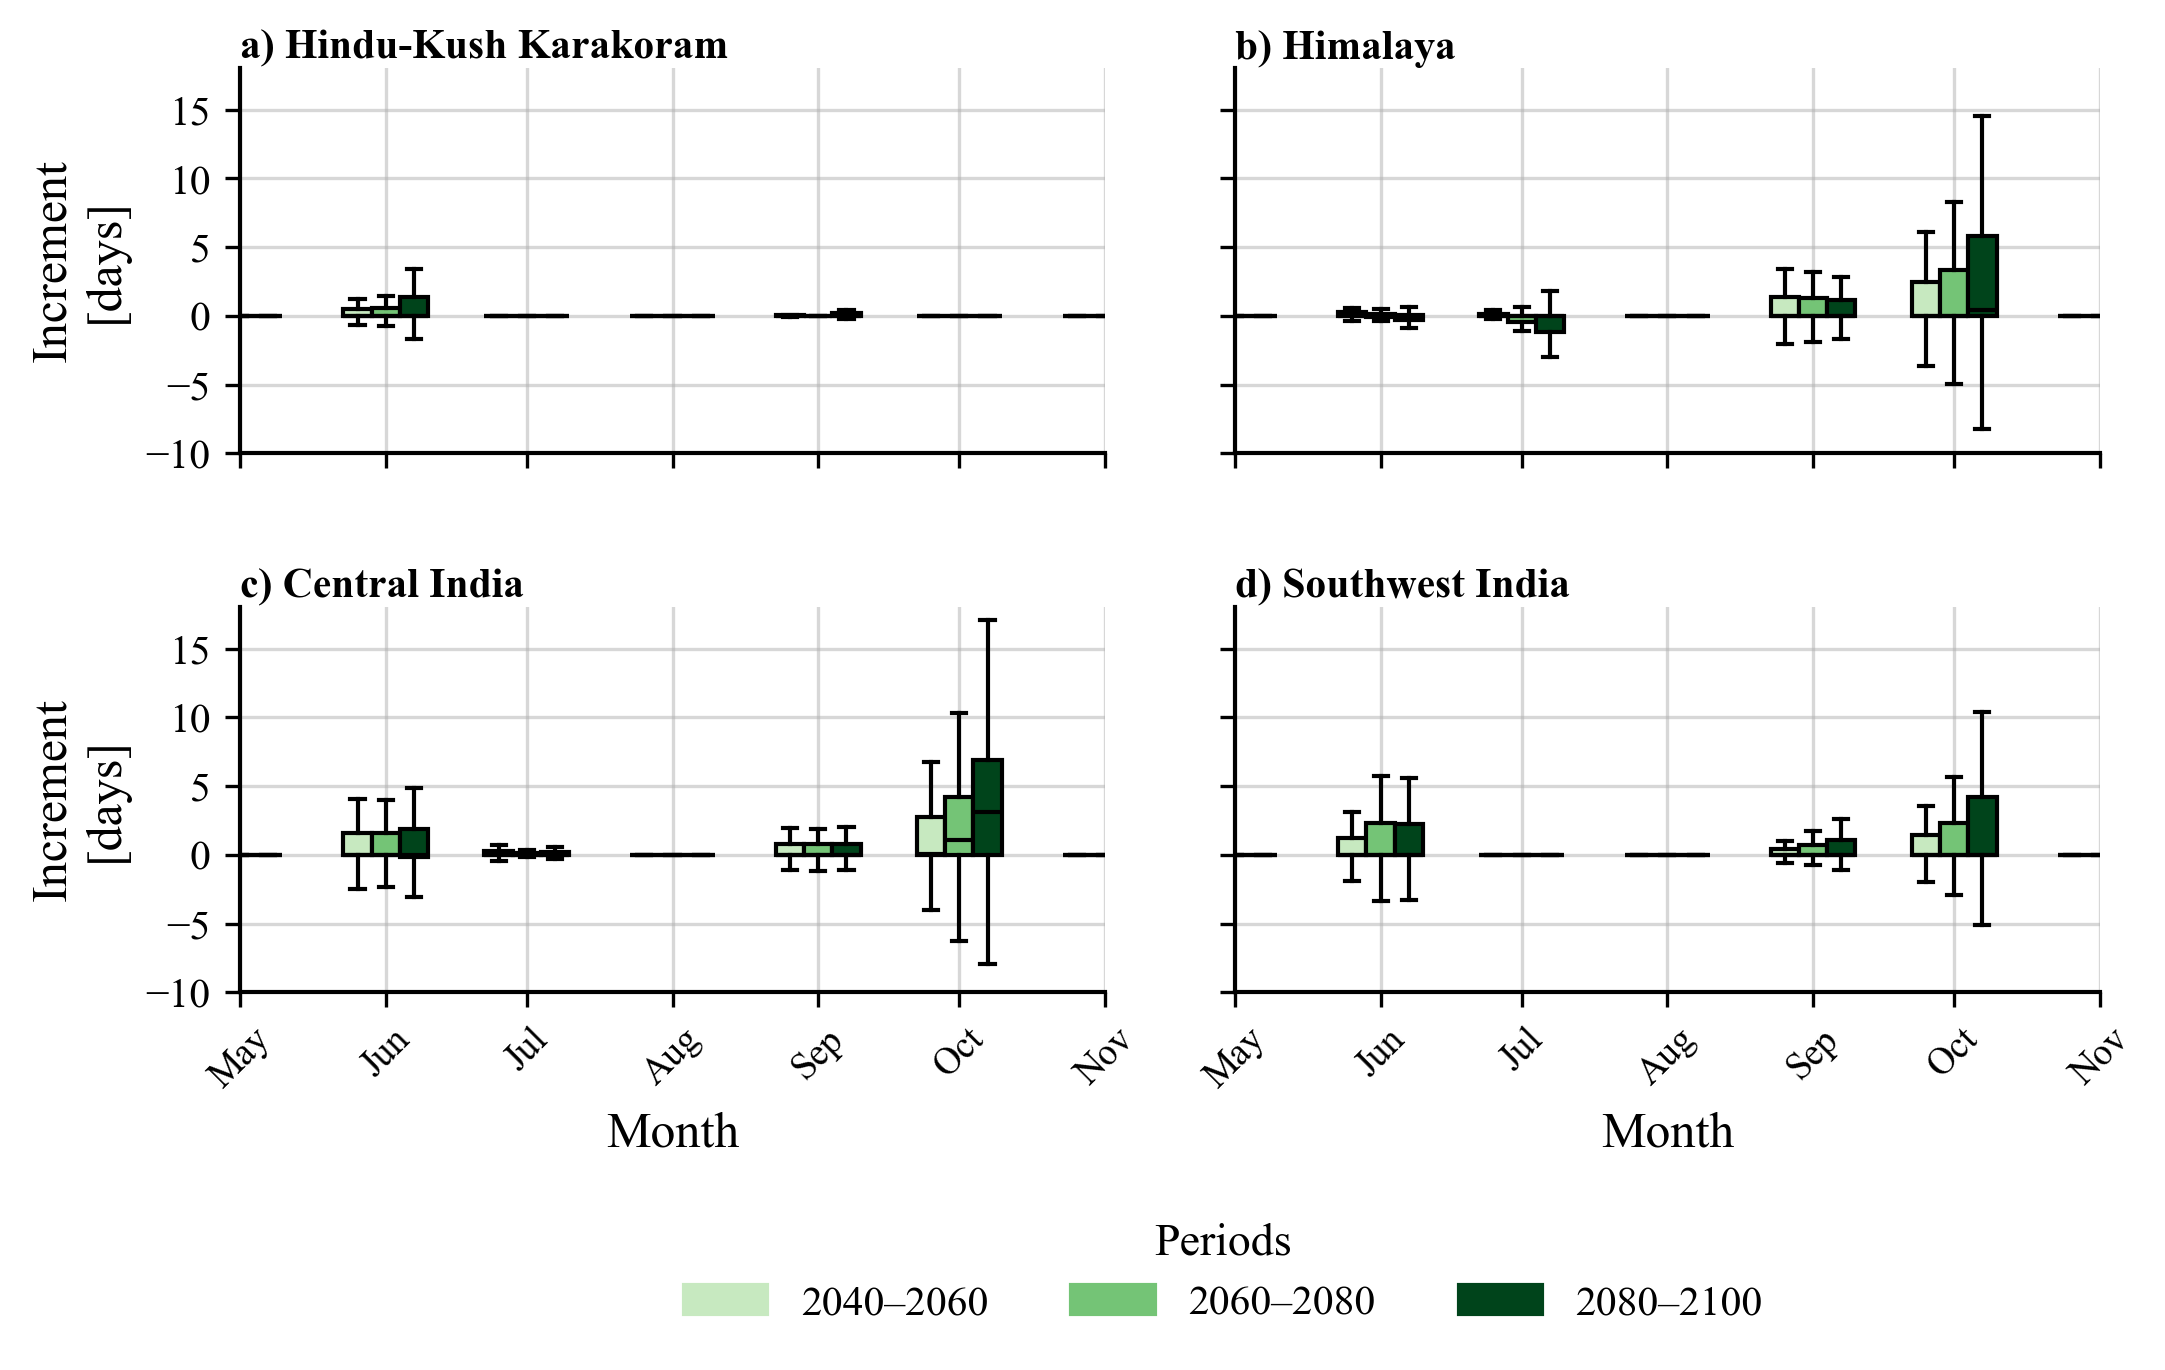
\includegraphics[width=0.9\textwidth]{Chapter3/figs/monthly_increment_monsoon.png}
    \caption{Projected monthly change in the number of days classified as monsoon during three future periods, relative to the 1970--2000 climatology. Each panel represents one of the four subregions, and the distributions combine grid points and models included in the SMME.}
    \label{fig:monthly_increment_monsoon}
\end{figure}

The winter season shows an opposite tendency. Its duration decreases across much of the subcontinent, particularly in Central and Southern India, where trends reach approximately $-1.5$ days per decade (Figure~\ref{fig:spatial_trends}b). Although negative trends also appear in the mountain regions, they are less spatially coherent and are frequently not statistically significant.

Central India experiences the largest change, with a projected loss of up to ten winter days by the end of the century (Figure~\ref{fig:seasonal_increment}c). The contraction becomes more pronounced after 2040 and is concentrated mainly in December and January. The Himalaya shows a similar but weaker signal, with a reduction of approximately five winter days by 2100 (Figure~\ref{fig:seasonal_increment}b). In contrast, neither Southwest India nor the Hindu Kush--Karakoram exhibits a coherent regional change. Over Southwest India, local trends have opposing signs, while projections over the Hindu Kush--Karakoram remain limited by low model agreement and historical skill.

The projected shortening should not be interpreted simply as the direct effect of increasing temperature. The preprocessing applied in this framework removes long-term changes in the mean and variance of the individual climate variables. The classification therefore responds to changes in their intra-annual distribution and relationships rather than to the mean warming trend itself. In Central India, for example, the winter class is defined primarily by precipitation and low-level zonal circulation rather than by temperature alone (Table~\ref{tab:feature_importance}). The loss of winter days consequently indicates that the multivariate conditions associated with winter become less frequent or less distinct from those of the surrounding seasons.

Temperature plays a larger role in identifying winter over the Himalaya and Hindu Kush--Karakoram, where it accounts for approximately 43\% and 44\% of relative feature importance, respectively. Nevertheless, the strong warming projected over these regions does not produce a coherent winter shortening over the Hindu Kush--Karakoram. This result further illustrates that changes in a single variable do not necessarily correspond to changes in the multivariate seasonal state captured by the classification.

\begin{figure}[H]
    \centering
    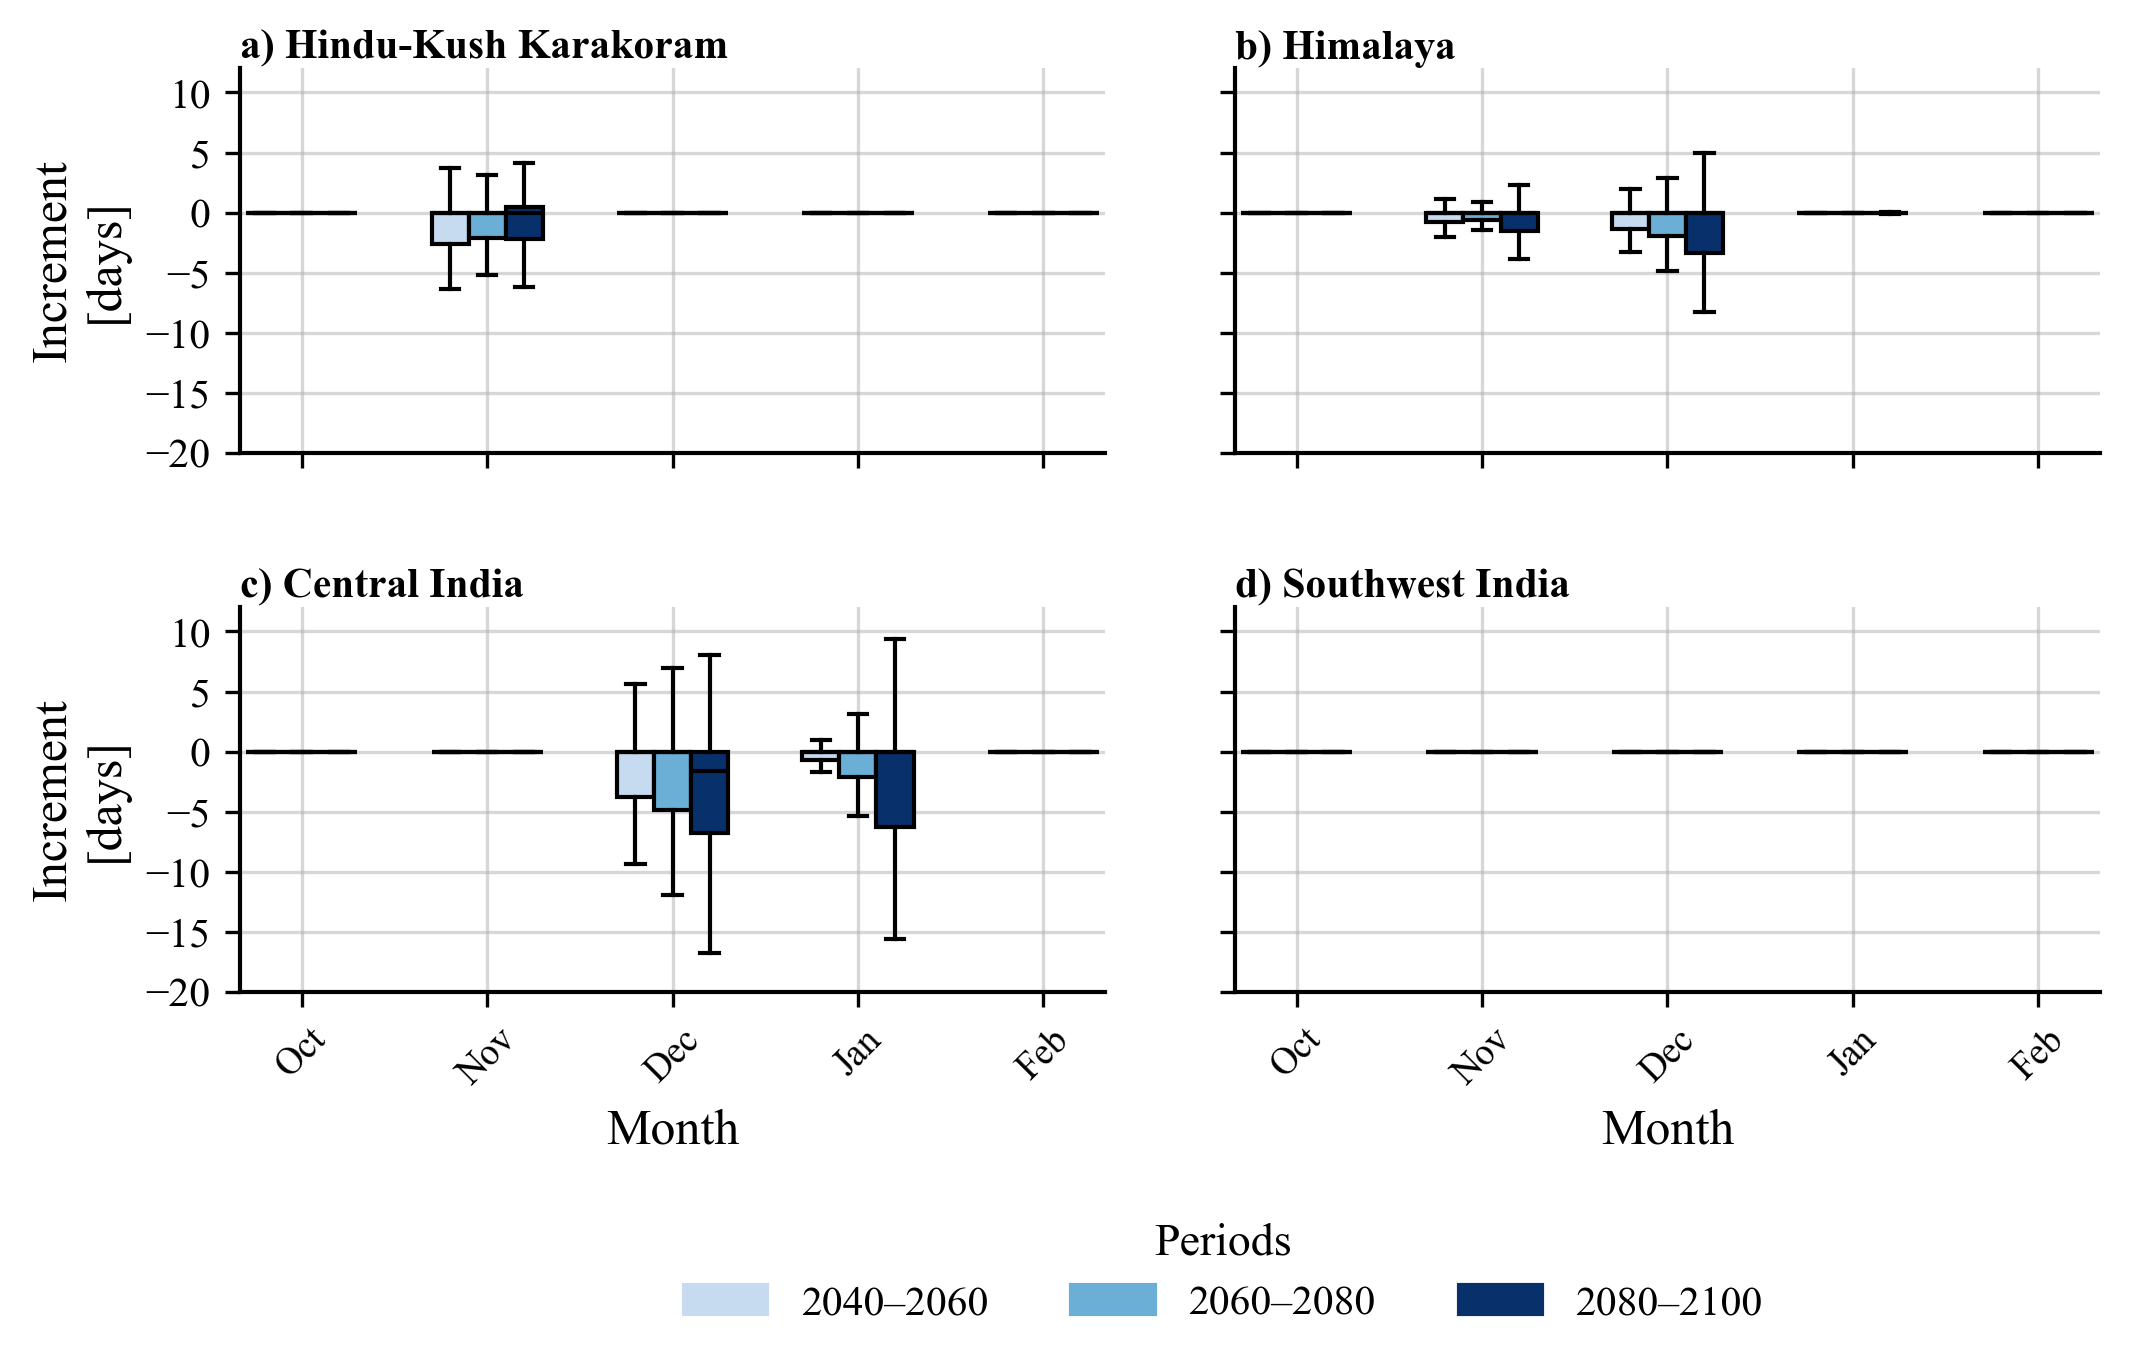
\includegraphics[width=0.9\textwidth]{Chapter3/figs/monthly_increment_winter.png}
    \caption{Projected monthly change in the number of days classified as winter during three future periods, relative to the 1970--2000 climatology. Each panel represents one of the four subregions, and the distributions combine grid points and models included in the SMME.}
    \label{fig:monthly_increment_winter}
\end{figure}

Overall, the projections indicate that seasonal changes are not uniform shifts of the annual cycle. The monsoon tends to persist later into the year, while the contraction of winter is concentrated in specific months and varies substantially across regions. 



\section{Discussion}

This chapter started from a simple question: how can information about meteorological seasons be inferred from climate data, given their heuristic nature? Seasons are familiar concepts, but climate datasets do not contain explicit labels indicating where one season ends and another begins. Their identification requires continuous and multivariate atmospheric conditions to be translated into discrete and interpretable categories.

The results show that this translation can be performed using a relatively simple Machine Learning framework. The seasonal partition learned from ERA5 broadly reproduces the annual cycle conventionally used to describe the Indian climate, including the monsoon, winter, and the two transition periods. Its consistency with the IMD monsoon patterns suggests that the clustering captures recognizable climatic structures rather than merely producing a mathematically convenient separation of the data. The analysis of the classifier also shows that these structures emerge from different combinations of temperature, precipitation, and circulation, depending on the season and region.

The resulting definitions should not be interpreted as replacements for the operational criteria adopted by the IMD. Operational definitions are designed to identify specific events and respond to established institutional needs. The framework developed here instead provides a multivariate description of the complete annual cycle. Its value lies in producing a consistent seasonal representation that can be applied beyond the dataset from which it was derived.

This transferability was tested by applying the ERA5-based definitions to CMIP6 simulations. The results show that the approach performs well where climate models reproduce the dominant seasonal regimes, particularly in Central and Southwest India. Its performance is less robust over the Himalaya and Hindu Kush--Karakoram, where complex topography and the interaction of different circulation systems remain challenging for global climate models. This indicates that the reliability of the information produced by the algorithm cannot be evaluated independently of the quality of the underlying climate data.

For this reason, model skill was incorporated directly into the analysis of future changes. The resulting projections indicate a lengthening of the monsoon over large parts of Central and Southern India, mainly because of delayed withdrawal, together with a shortening of winter concentrated in December and January. These changes do not represent simple shifts of fixed calendar boundaries. Instead, they describe changes in the persistence and timing of the multivariate atmospheric conditions associated with each seasonal regime.

At the same time, these results illustrate that climate data do not contain a single, universally valid definition of a season. For example, the monsoon lengthening identified here differs from the shortening found using a large-scale circulation indicator by \citet{cheng_shorter_2025}. The two approaches describe different components of the monsoon system: one identifies the persistence of regional hydroclimatic conditions, while the other describes changes in large-scale circulation. The information obtained from climate data therefore depends on the variables, scale, and definition adopted.

The data-driven character of the framework should consequently not be understood as the absence of assumptions. The number of seasons, the input variables, the temporal smoothing, and the normalization procedure are all part of the definition being constructed. Machine Learning avoids prescribing separate thresholds for individual variables, but it does not remove the scientific choices required to formulate the problem. These choices must remain transparent if the resulting indicators are to be interpreted correctly.

Within the Climate Services value chain, the framework performs an inference step: it transforms large volumes of climate data into indicators of seasonal timing and duration. These indicators are more accessible and comparable than the original multivariate datasets, but they are not yet decision-relevant knowledge. A delayed monsoon withdrawal, for example, acquires practical meaning only when connected to a specific context such as crop calendars, reservoir management, or flood risk.

The case study therefore demonstrates both the potential and the limits of AI in transforming climate data into information. The contribution of the algorithm does not lie simply in detecting patterns, but in producing a representation that can be validated physically, transferred across datasets, and evaluated according to the reliability of the underlying models. These conditions are essential for algorithmic outputs to become credible climate information and, through further contextualization, contribute to decision-relevant knowledge.